\documentclass{beamer}
%[aspectratio=169]   \usepackage[czech]{babel}
\usepackage{apo-lecture}
\usepackage{pdfpages}
\usepackage{pdfcomment}
\usepackage{listings}
\usepackage{array,multirow}

\subtitle{Lekce 04. Hierarchie paměti}
\author{Pavel Píša \phantom{xxxxxxx} Petr Štěpán \\ \small\texttt{pisa@fel.cvut.cz}\phantom{xxxx}\small\texttt{stepan@fel.cvut.cz}}
\begin{document}

\maketitle

\section{Paměť úvod}

\begin{frame}[fragile]
\frametitle{Motivace}

\begin{columns}
\begin{column}{0.45\textwidth}
Algoritmus A\\
\begin{minted}{c}
int matrix[N][N];
int main() {
  long int i, j, sum1 = 0;
  for(i=0; i<N; i++)
    for(j=0; j<N; j++)
      sum1 += matrix[i][j];
}
\end{minted}
\end{column}
\hfill
\begin{column}{0.45\textwidth}
Algoritmus B\\
\begin{minted}{c}
int matrix[N][N];
int main() {
  long int i, j, sum1 = 0;
  for(i=0; i<N; i++)
    for(j=0; j<N; j++)
      sum1 += matrix[j][i];
}
\end{minted}
\end{column}
\end{columns}
\bigskip
Oba dva programy vypadají velmi podobně. 

Program A prochází pole po řádcích, program B prochází pole po sloupcích.
\bigskip

Bude se nějak lišit doba výpočtu?

\end{frame}

\begin{frame}[fragile]
\frametitle{Motivace}

\begin{columns}
\begin{column}{0.45\textwidth}
Algoritmus A\\
\begin{minted}{c}
int matrix[N][N];
int main() {
  long int i, j, sum1 = 0;
  for(i=0; i<N; i++)
    for(j=0; j<N; j++)
      sum1 += matrix[i][j];
}
\end{minted}
\end{column}
\hfill
\begin{column}{0.45\textwidth}
Algoritmus B\\
\begin{minted}{c}
int matrix[N][N];
int main() {
  long int i, j, sum1 = 0;
  for(i=0; i<N; i++)
    for(j=0; j<N; j++)
      sum1 += matrix[j][i];
}
\end{minted}
\end{column}
\end{columns}
\bigskip

\begin{tabular}{|l|l|l|}\hline
N & A & B \\\hline
100000 & 12.791328s &138.047563s \\\hline
10000 & 0.126945s &0.486535s \\\hline
1000 & 0.001329s &0.001756s \\\hline
100 & 0.000083s &0.000094s \\\hline
\end{tabular}
\end{frame}

\begin{frame}
\frametitle{Co je paměť}

\centering

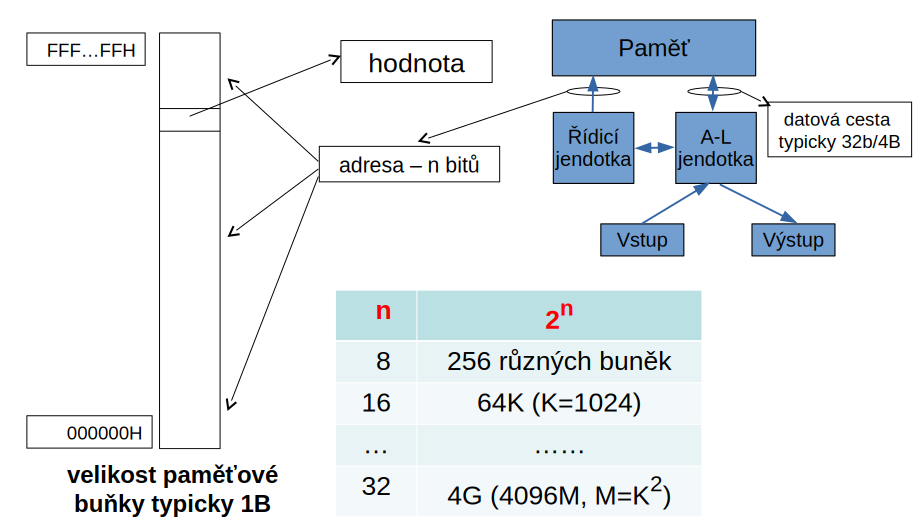
\includegraphics[width=.95\linewidth]{addr-space.pdf}

\end{frame}

\begin{frame}
\frametitle{Co je paměť -- popis}

Paměť :
\begin{itemize}
\item je pole adresovatelných buněk
\begin{itemize}
\item buňky mají shodnou šíři - většinou 8 bitů (byte) nebo jejich násobek
\end{itemize}
\item velikost fyzického adresového prostoru je omezena počtem bitů adresy, kterou je CPU schopno nastavit na paměťové sběrnici, tedy kolik bitů lze použít k adresování paměti. Pro organizaci po bytech pak
\begin{itemize}
\item 16 bitů adresy umožňuje maximálně 64KiB velkou paměť
\item 32 bitů adresy umožňuje maximálně 4GiB velkou paměť
\item 37 bitů adresy (maximum procesoru Intel Core  i9-13900K, pak záleží ještě na základní desce) maximálně 128 GiB velkou paměť
\end{itemize}
\item typ přístupu:
\begin{itemize}
\item k vnitřní paměti počítače lze přistupvat v náhodném pořadí (= random access -- RAM)
\item některé externí paměti (např. magnetopásková paměť využívaná pro zálohování -- levnější než HDD a SSD) umožňjí pouze sekvenční přístup, tedy čtení a zápis bajtů po sobě
\item pro HDD, SSD, Flash je možný přítup po celých blocích, u SSD/Flash je zápis bloku možný vždy jednou do smazání po velkých celcích
\end{itemize}
\end{itemize}

\end{frame}

\begin{frame}
\frametitle{Polovodičových paměti -- terminologie}

\begin{description}
 \item[Adresa] vstup, který vybírá svojí hodnotou jednu konkrétní buňku paměti
 \item[Hodnota] vlastní informace
 \item[stavová data] volitelně další informace (třeba o platnosti hodnoty, redundanci pro opravení chyb, apod.)
\end{description}

Parametry pamětí:

\begin{description}
  \item[Vybavovací doba paměti] (latence) kritický parametr. Délka časového intervalu mezi objevením se požadavku a okamžikem, kdy jsou data k dispozici.
  \item[Doba přístupu] vybavovací doba + obnovení obsahu po destruktivním čtení připadně doba, kdy lze zadat další požadavek
  \item[Propustnost] výkonový parametr. Schopnost zpracovat uvedené množství za jednotku času.
\end{description}

\end{frame}

\section{Technologie polovodičové paměťi}

\begin{frame}
\frametitle{Druhy paměti}

Paměti dělíme podle možností zápisu na:
\begin{itemize}
\item \textbf{ROM} (Read-Only Memory) paměti ze kterých lze pouze číst, řadíme sem i paměti typu EEPROM (Electrically Erasable Programmable Read-Only Memory), které lze omezeně smazat vysokým napětím a pak tam zapsat nové údaje, při normálním provozu nejde do paměti zapsat.
\item \textbf{RAM} (Random Access Memory) také RWM (Read-Write Memory) lasické paměti určené pro čtení a zápis libovolné buňky v libovolném pořadí -- Random Access.
\end{itemize}

Paměti lze dělit i podle toho, zda data jsou uchována po vypnutí napájení:
\begin{itemize}
\item \textbf{Permanentní} (Non-volatile) paměť nepotřebuje k udržení informace napájení - např. Flash, EEPROM, EPROM, ROM, feromagnetické paměti, HDD, SSD, 3D-X Point -- Intel Optane Memory
\item \textbf{Volatilní} (Volatile) například paměť DDR SDRAM, SRAM, cache v klasickém počítači, k udržení informace je potřeba nepřetržité napájení a obnova dat.
\end{itemize}
\end{frame}

\begin{frame}
\frametitle{Konstrukce paměti}

Podle kontrukce dělíme paměti RAM (RWM) na:
\bigskip

\begin{tabular}{m{0.8cm}m{6cm}m{4cm}}
SRAM & Statická RAM -- veličina reprezentující hodnotu má v čase konstatní hodnotu. Typicky dva do smyčky zapojené invertory. Více součástek dražší paměť, nemusí se obnovovat uložená informace, potřebuje pouze napájení & 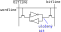
\includegraphics[width=3.8cm]{sram.pdf} \\ 
\phantom{x} & & \\
DRAM & Dynamická RAM -- veličina mění v čase svoji hodnotu. Typicky kondezátor, který se samovolně vybíjí a je proto nutné informaci obnovovat v pravidelných časech. Pouze kondenzátor a tranzistor -- levné, zabere méně prostoru. & 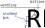
\includegraphics[width=3.2cm]{dram.pdf}\\
\end{tabular}

\end{frame}

\begin{frame}
\frametitle{Detail paměťové statické paměti -- SRAM}

\hbox{
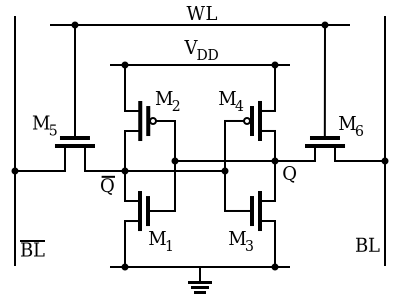
\includegraphics[width=0.4\linewidth]{sram-6t-cell.pdf}\hspace{0.1\linewidth}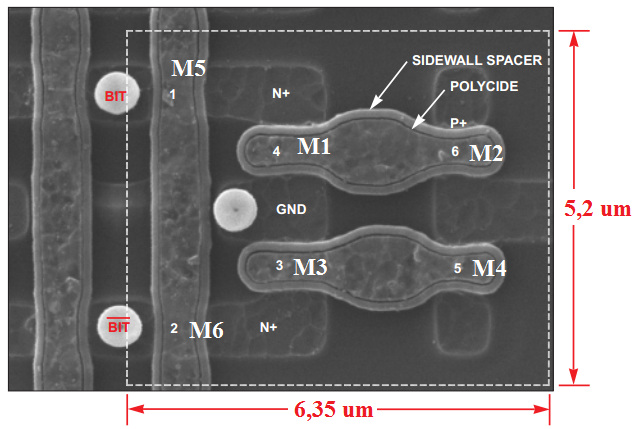
\includegraphics[width=0.4\linewidth]{fig/sram-cell.jpg}
}

\begin{itemize}
\item Plně statické zapojení (kladná zpětná vazba)
\item Pro udržení informace vyžaduje napájení (volatilní paměť)
\item Nevýhoda, potřebuje 6 tranzistorů, velká plocha
\item Čení, po výběru slova (world line -- WL) jsou data přenesena na příslušné nenapájené dráhy (bit line -- BL)
\item Při zápisu přes připojené bitové dráhy na log. 1 a log. 0 dojde k vnucení stavu vetším proudem než zajišťuje vnitřní smyčka
\end{itemize}

\end{frame}

\begin{frame}
\frametitle{Detail paměťové buňky dynamické paměti -- DRAM}

\hbox{
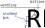
\includegraphics[width=0.4\linewidth]{dram.pdf}\hspace{0.1\linewidth}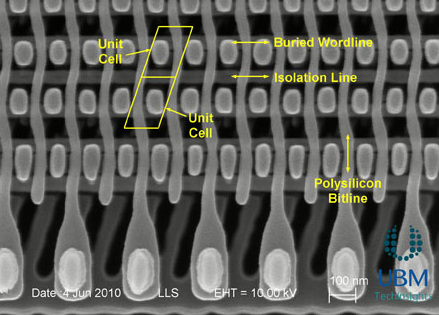
\includegraphics[width=0.4\linewidth]{fig/dram-cell.jpg}
}

\begin{itemize}
\item nMOS tranzistor představuje přepínač, který připojí (nebo ne) kondenzátor na vodič „bitline“. Připojení je řízeno vodičem „wordline“.
\item Proces čtení kondenzátor vybíjí. Proto musí být poté obnoven.
\item Občerstvování pamětí (refresh) – náboj se z kondenzátoru samovolně ztrácí. Nezbytná pracovní fáze dynamické paměti. Negativně ovlivňuje (prodlužuje) průměrnou vybavovací dobu.
\end{itemize}

\end{frame}

\begin{frame}
\frametitle{Paměťová matice -- základ}

\centering

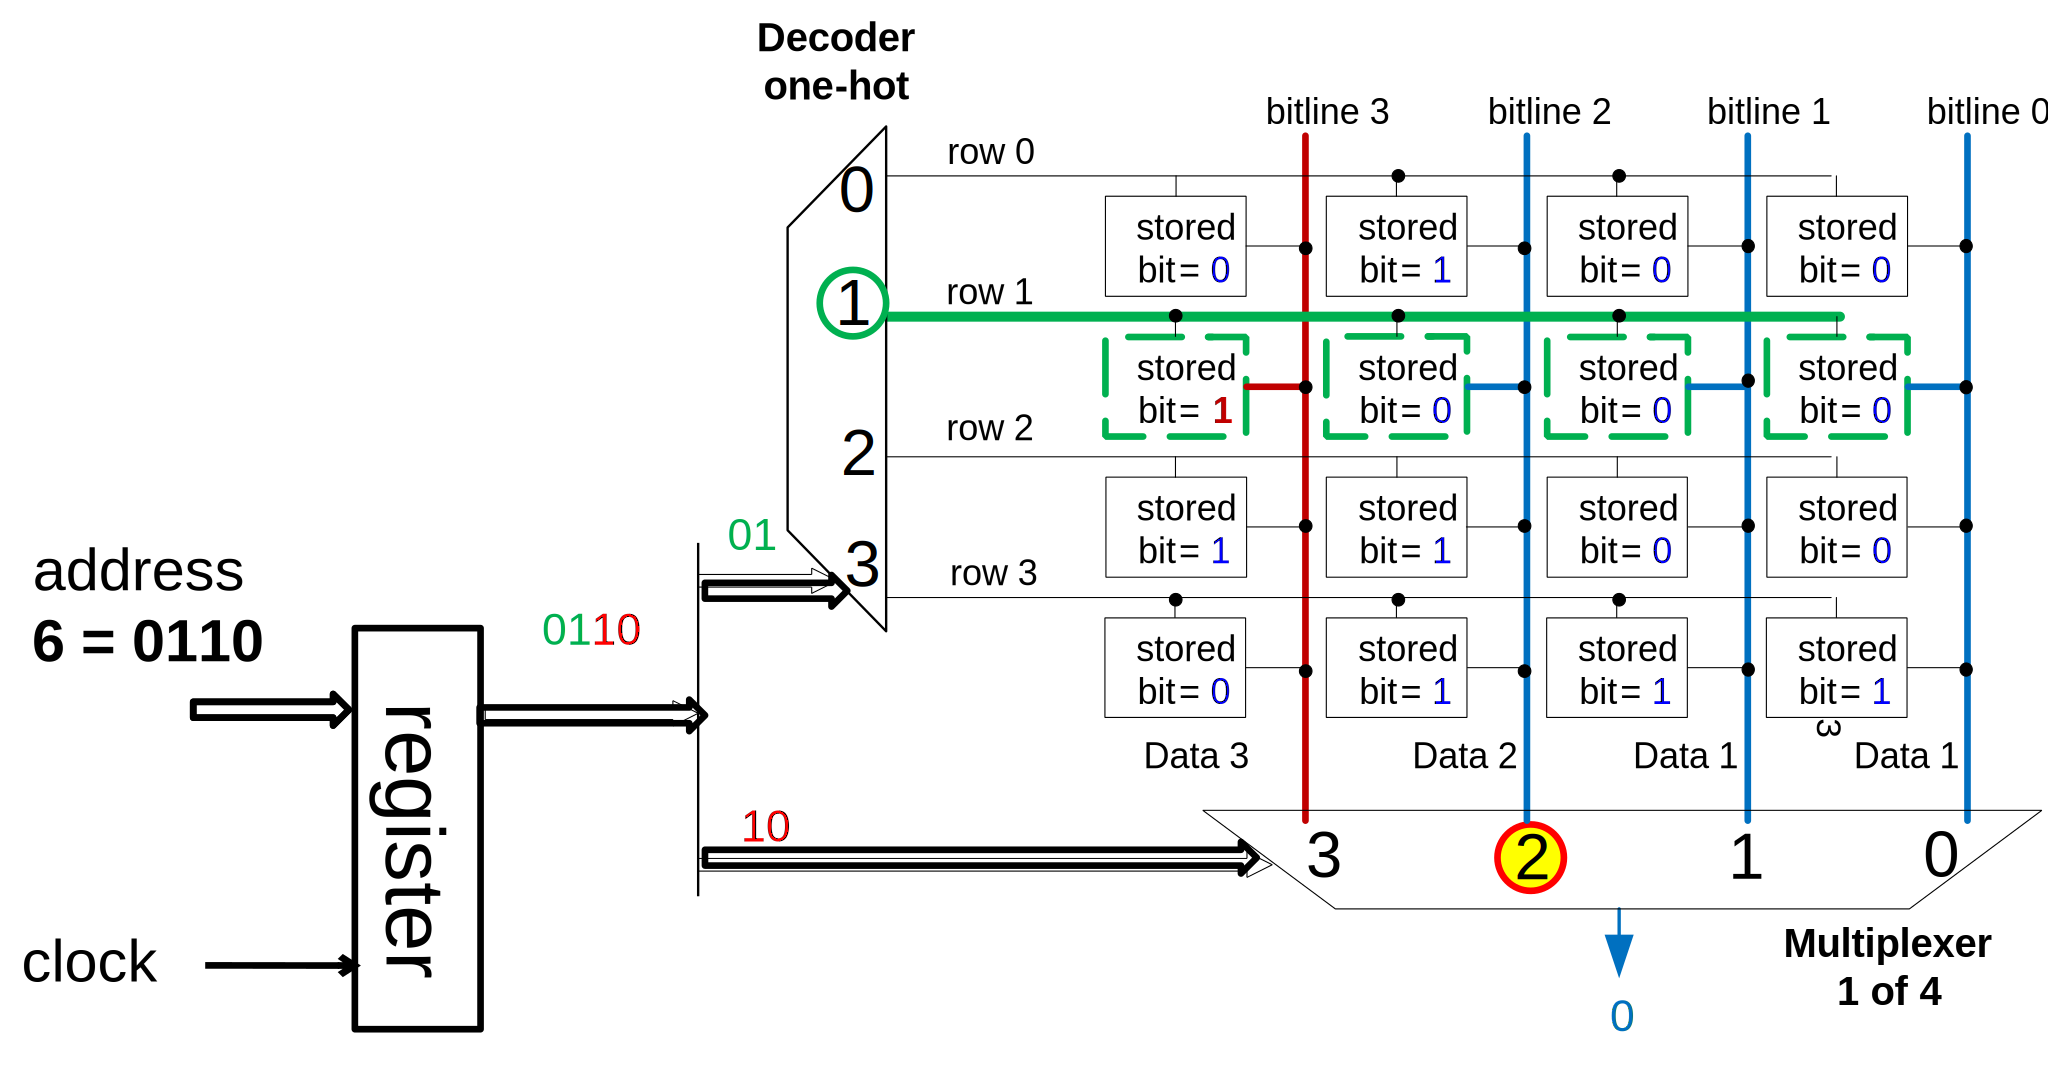
\includegraphics[width=1.0\linewidth]{ram-matrix.pdf}

\end{frame}

\begin{frame}
\frametitle{Moduly s dynamickou pamětí}

\centering

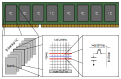
\includegraphics[width=0.85\linewidth]{sdram-dimm.pdf}

\end{frame}

\begin{frame}
\frametitle{Paměť v dnešních osobních počítačích}

{
\centering

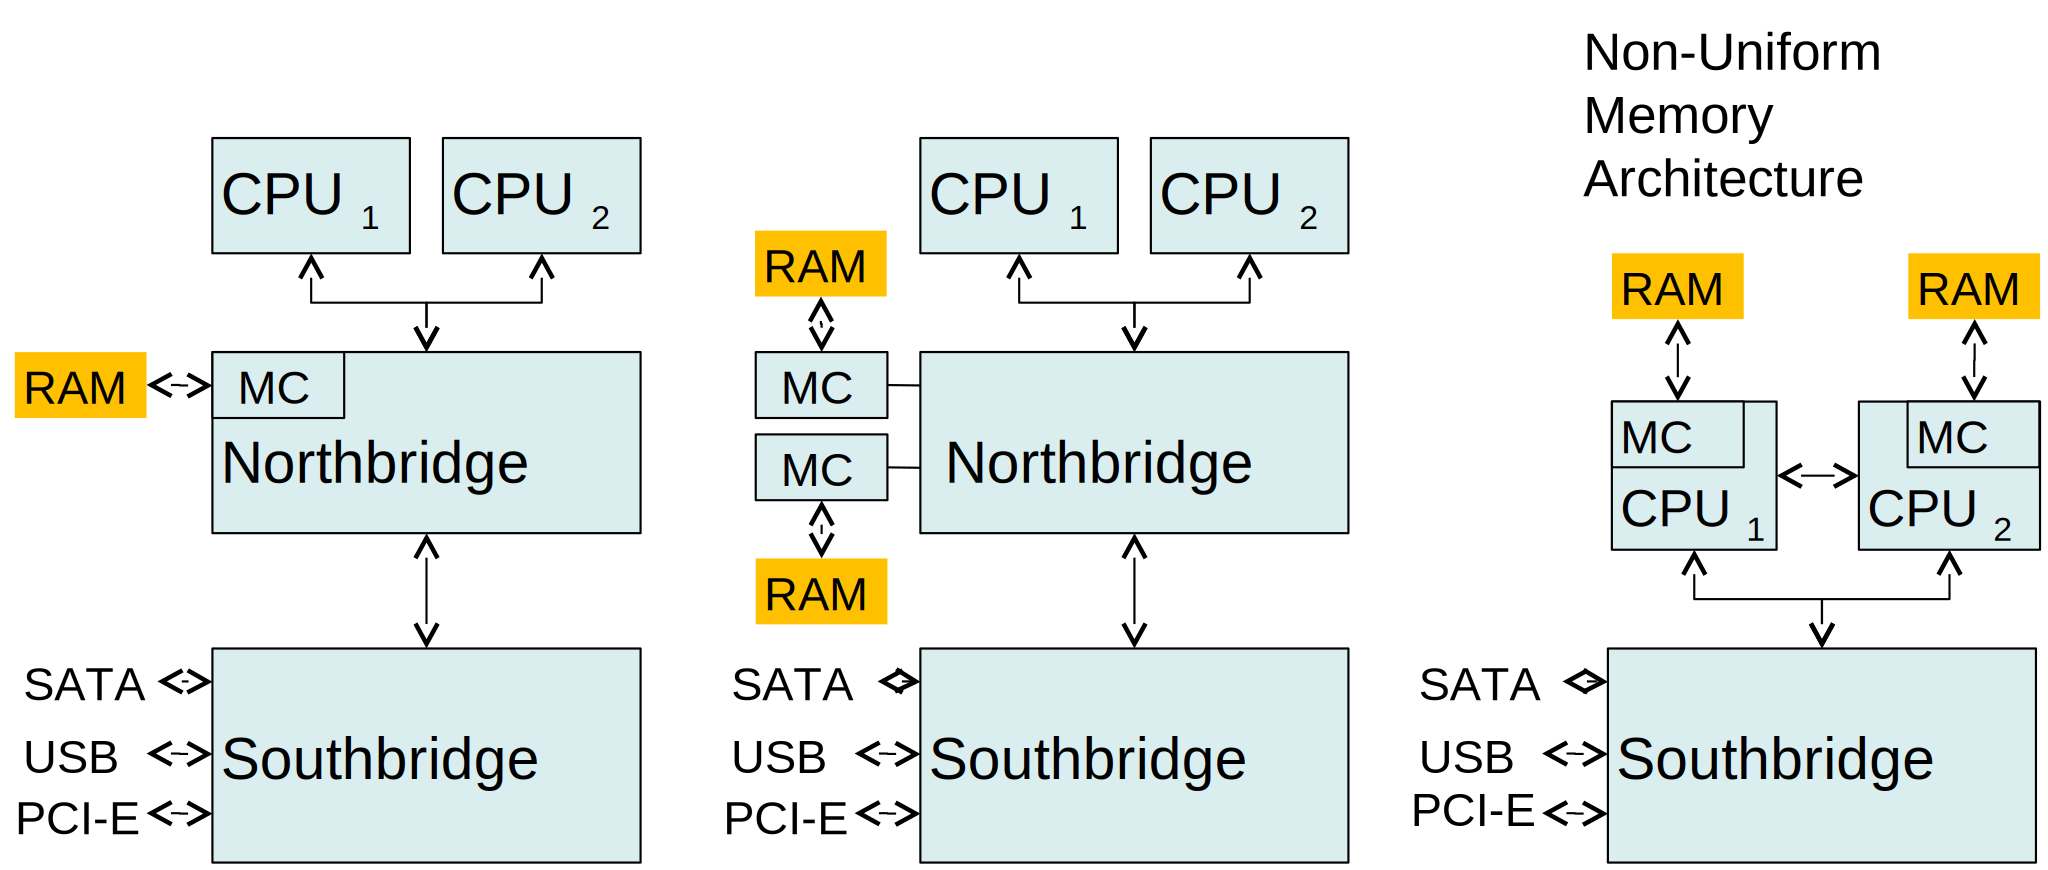
\includegraphics[width=0.85\linewidth]{pc-memory-to-numa.pdf}

}

\vskip 2mm

MC - Memory controller -- paměťový kontrolér zajišťuje řízení čtení a zápisů do SDRAM. Dále obstarává obnovu informace (refreshing) každé paměťové buňky jednou za 64 ms.

\end{frame}


\begin{frame}
\frametitle{Nejčastěji používané typy dynamických pamětí}

\begin{itemize}
\item \textbf{SDRAM} -- hodinová frekvence až 100 MHz, 2.5V, synchronní přenos dat na hodinové hraně
\item \textbf{DDR SDRAM} -- přenos dat na obou hodinových hranách, 2.5V, V/V hodiny až 100-200 MHz, 0.2-0.4 GT/s (miliard přenosů za skundu)
\item \textbf{DDR2 SDRAM} -- menší spotřeba, 1.8V, frekvence až 400 MHz, 0.8 GT/s
\item \textbf{DDR3 SDRAM} -- ještě nižsí spotřeba při 1.5V, frekvence až 800 MHz, 1.6 GT/s
\item \textbf{DDR4 SDRAM} -- 1.05 -- 1.2V,  V/V svěrnicové hodiny 1.2 GHz, 2.4 GT/s
\item \textbf{DDR5 SDRAM} -- 1.1V, až 6.4 GT/s
\end{itemize}

Všechny tyto druhy jsou převážně optializované na propustnost, nikoliv náhodný přístup, latence 20 až 35 ns.

\end{frame}


\begin{frame}
\frametitle{Rozdíl růstu výkonu procesorů a pěmětí}

\centering

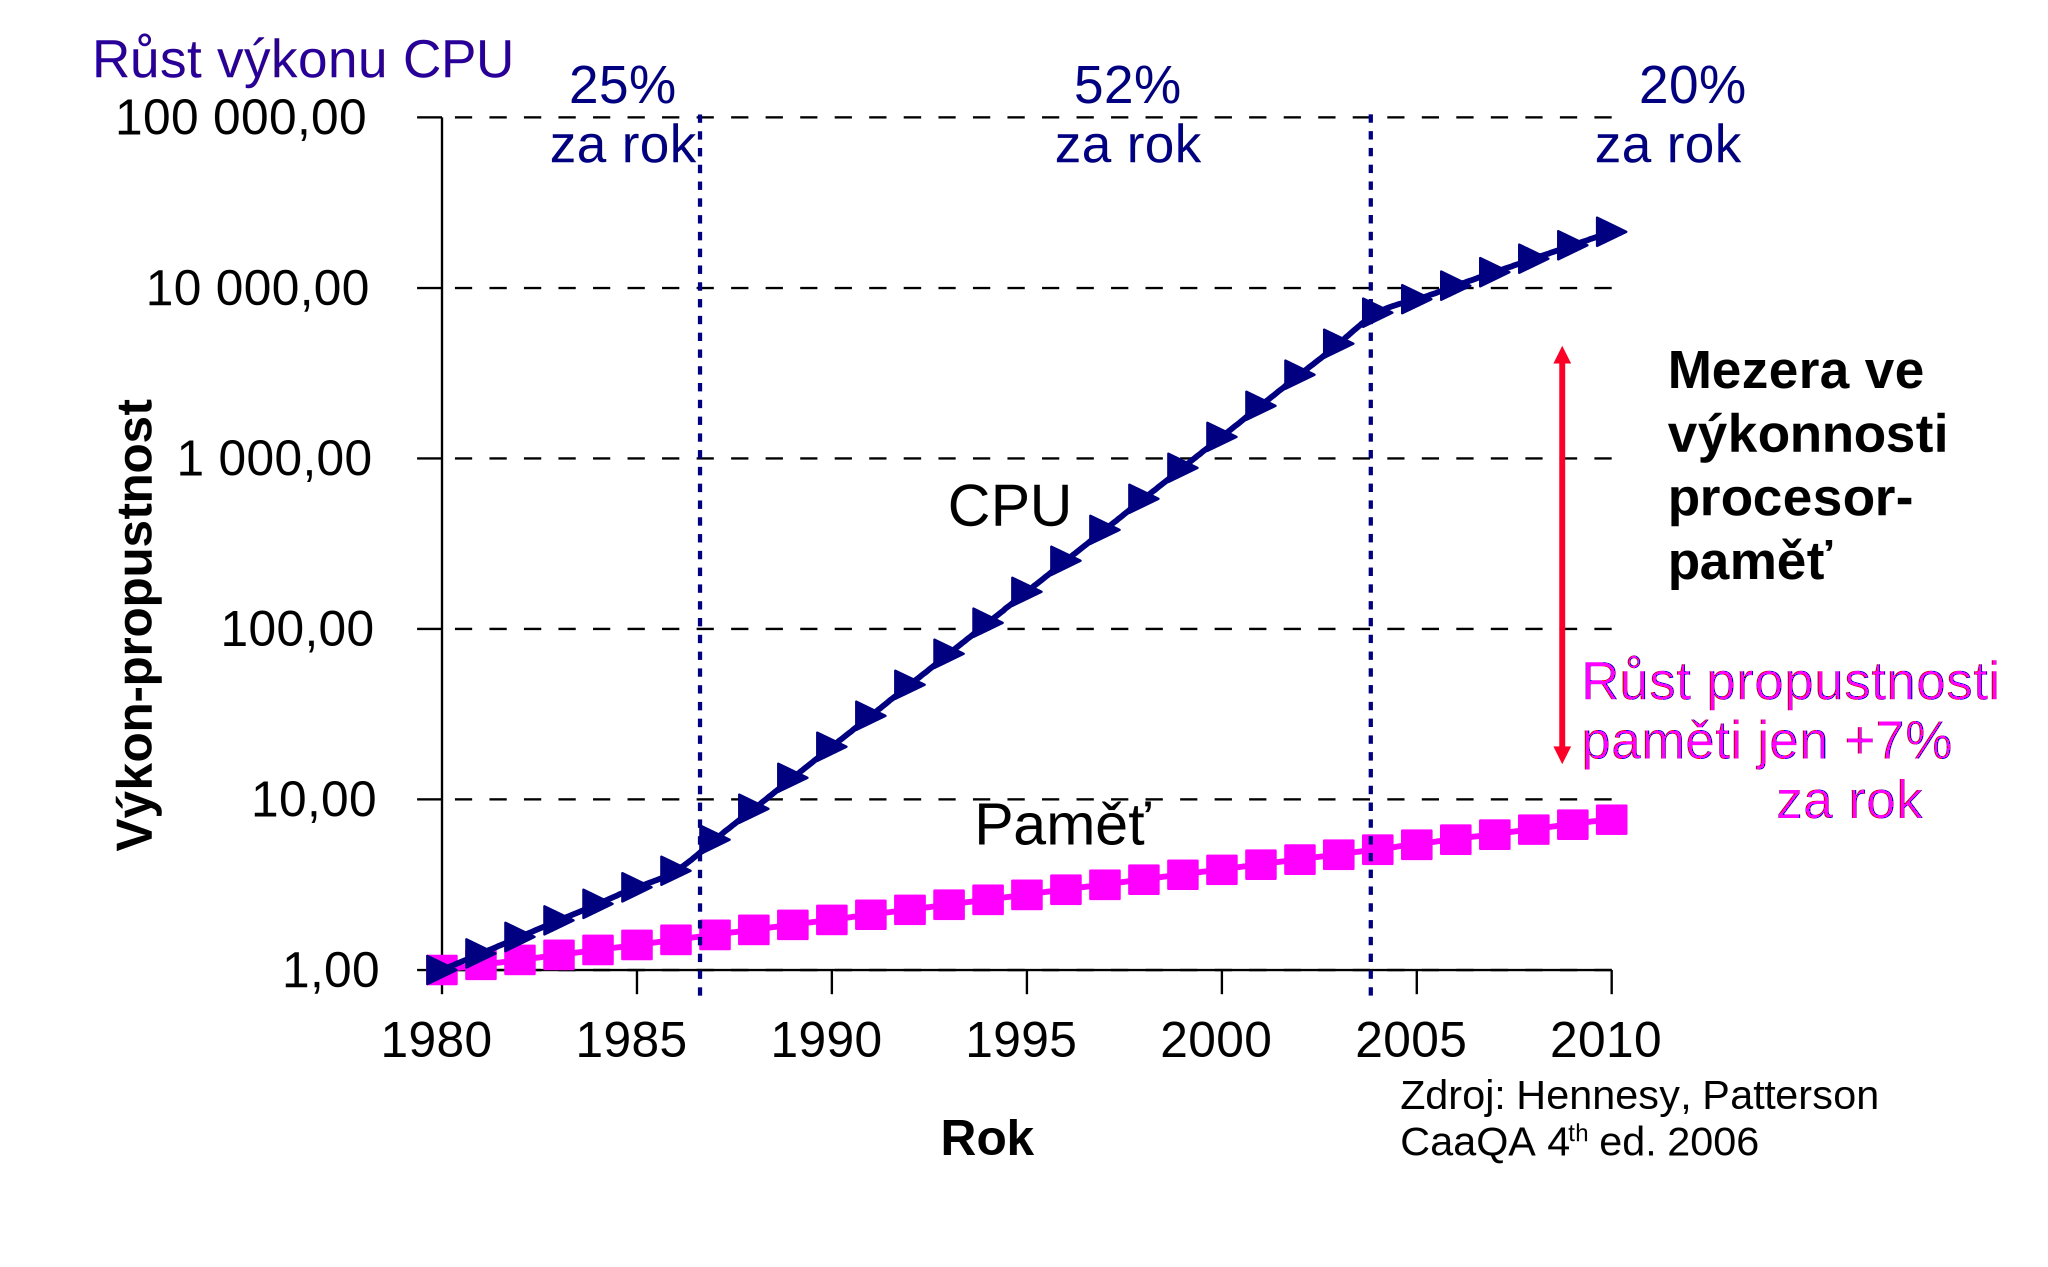
\includegraphics[width=1.0\linewidth]{memory-gap.pdf}

\end{frame}

\section{Zrychlení přístupu k datům, hierarchie, vyrovnávací paměť}

\begin{frame}
\frametitle{Paměťová hierarchie od registrů k SSD}

{
\centering

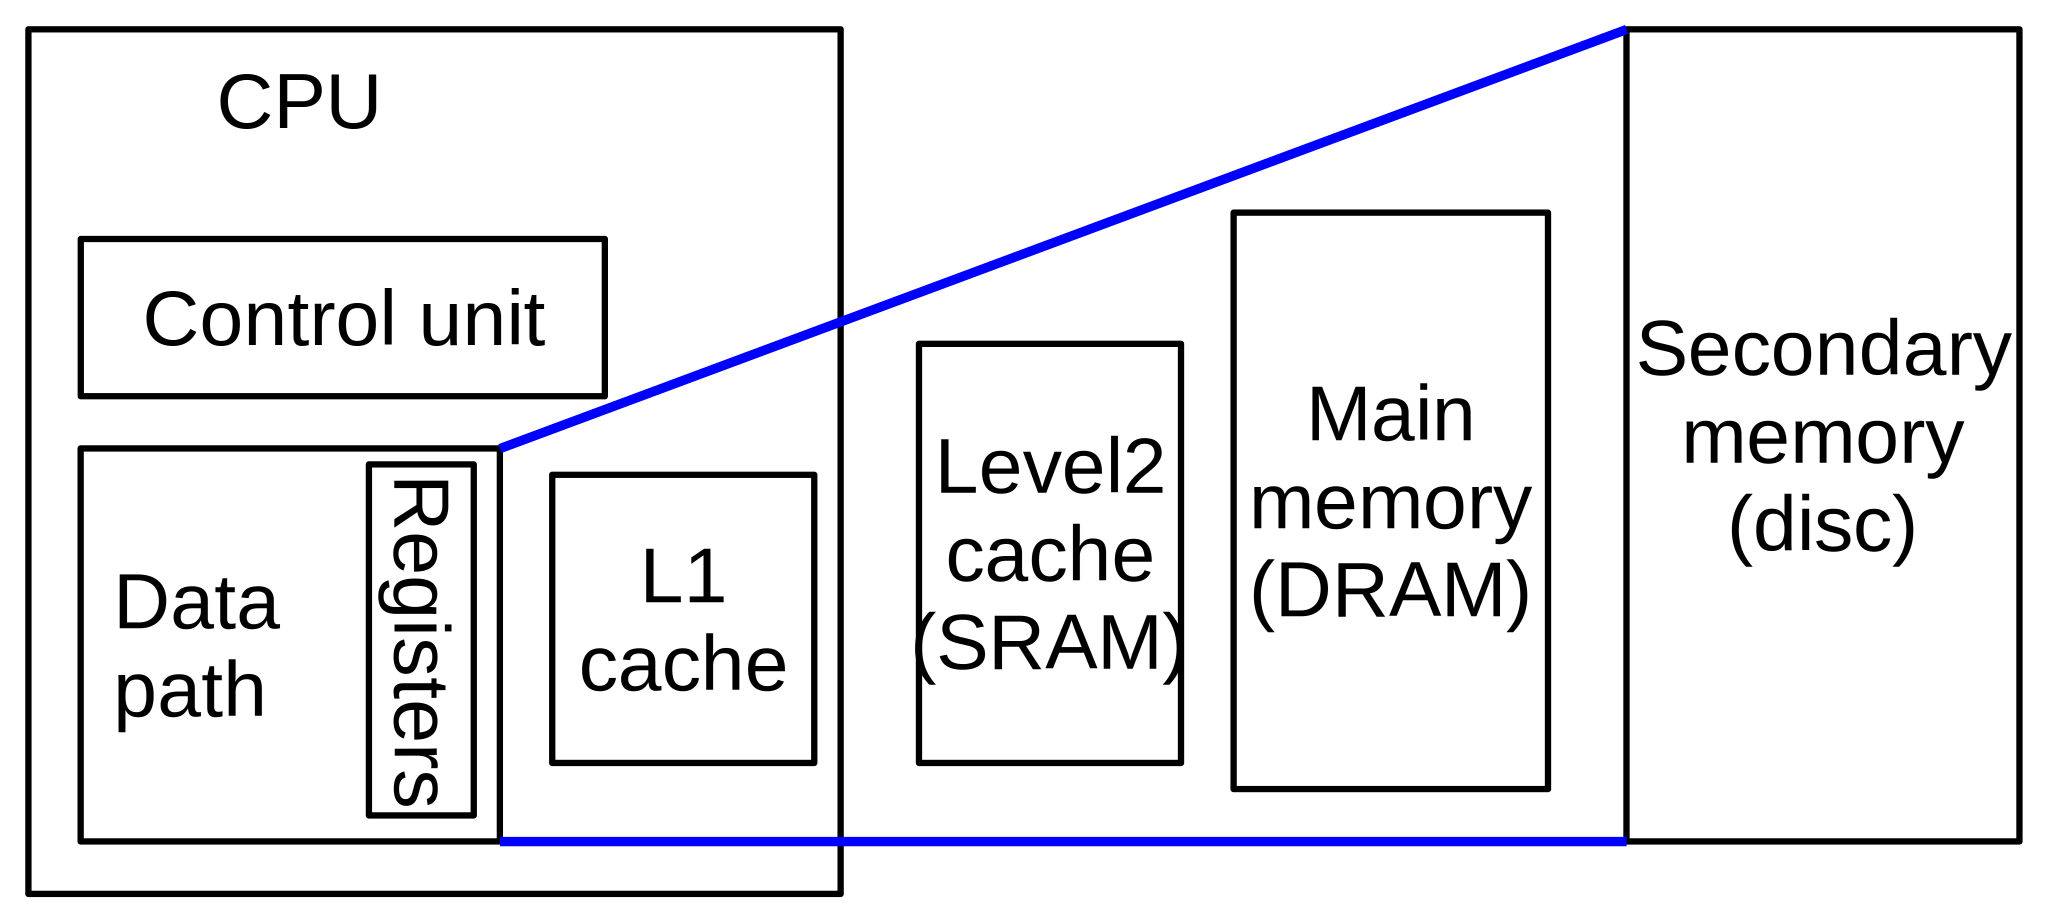
\includegraphics[width=0.65\linewidth]{mem-reg-to-disc.pdf}

}
\vskip 2mm

\begin{tabular}{l|llll}
Typ      & L1 SRAM   & Sync SRAM &  DDR3      & HDD \\
Velikost & 32kB      & 1 MB      &  16 GB     & 3TB \\
Cena     & 10 kč/kB  & 300 kč/MB &  123 kč/Gb & 1 kč/GB \\
Rychlost & 0.2...2ns & 0.5...8 ns/word & 15 GB/sec & 100 MB/sec \\
\end{tabular}

\vskip 2mm

Některá data mohou existovat ve více kopiích (úrovně, SMP).
Pro modifikaci dat je potřeba mechanizmů pro udržení koherence slov a konzistence datových struktur.

\end{frame}

\begin{frame}
\frametitle{Paměťová hierarchie -- základní principy}

\begin{itemize}
\item Programy/procesy přistupují v daném okamžiku jen k malé části svého adresového prostoru 
\item \textbf{Časová lokalita}
\begin{itemize}
\item Položky, ke kterým se přistupovalo nedávno, budou zapotřebí brzy znovu.
\item Příklad: programová smyčka, proměnné instrukcí.
\end{itemize}
\item \textbf{Prostorová lokalita}
\begin{itemize}
\item Položky poblíž právě používaným budou brzy zapotřebí také. 
\item Příklad: sekvenční přístup ke kódu (paměť programu), datová pole (paměť dat).
\end{itemize}
\end{itemize}
Princip se využívá jak v algoritmech (lokální proměnné), kompilátorech (přesun do registrů), na úrovni pamětí (automaticky), operačního systému (přesun z disku do paměti) případě opět programově, čtení a zápisy do souborů.
\end{frame}

\begin{frame}
\frametitle{Skryté paměti -- cache}

\begin{itemize}
\item je označení pro vyrovnávací paměť používanou ve výpočetní technice
\item Zařazujeme ji mezi dva subsystémy s různou rychlostí. Vyrovnává se jí rychlost přístupu k informacím.
\item Účelem skryté paměti je urychlit přístup k často používaným datům na „pomalých“ médiích jejich překopírováním na média rychlá.
\item Většinou z velké části pracuje automaticky a přispůsobuje se aktuální potřebě programu.
\item Přesto je nutné o její existenci vědět a často potřebuje servisní obsluhu na úrovni operačního systému a v něktěrých případech i programů.
\item Při nepromyšlené volbě datových struktur a algoritmů se její efekt ztrácí.
\end{itemize}

\end{frame}

\begin{frame}
\frametitle{Skryté paměti -- terminologie}

\begin{itemize}
\item \textbf{Cache hit} (zásah) pojmenování situace, kdy požadovaná hodnota ve skryté paměti (cache) je.
\item \textbf{Cache miss}, opak, \textbf{výpadek}, data v cache ještě nejsou.
\item \textbf{Cache line} (řádka) nebo \textbf{Cache block} – základní kopírovatelná jednotka mezi hierarchickými úrovněmi. 
\item V praxi se velikost \textbf{Cache} Line pohybuje od 8B do 1KB, typicky 64B.
\item \textbf{Hit rate} -- počet paměťových přístupů obsloužených danou úrovní cache dělený všemi přístupy
\item \textbf{Mis rate} -- poměr přístupů, které je potřeba obsloužit z pomalejší paměti = 1 - Hit rate
\item \textbf{Average Memory Access Time} (AMAT) $$AMAT = Hit Time + Miss Rate \times Miss Penalty$$
\item AMAT pro víceúrovňovou cache lze spočítat rekurzivní aplikací výšeuvedeného vztahu
\end{itemize}

\end{frame}

\begin{frame}
\frametitle{Skryté paměti -- realizace}
{
\centering

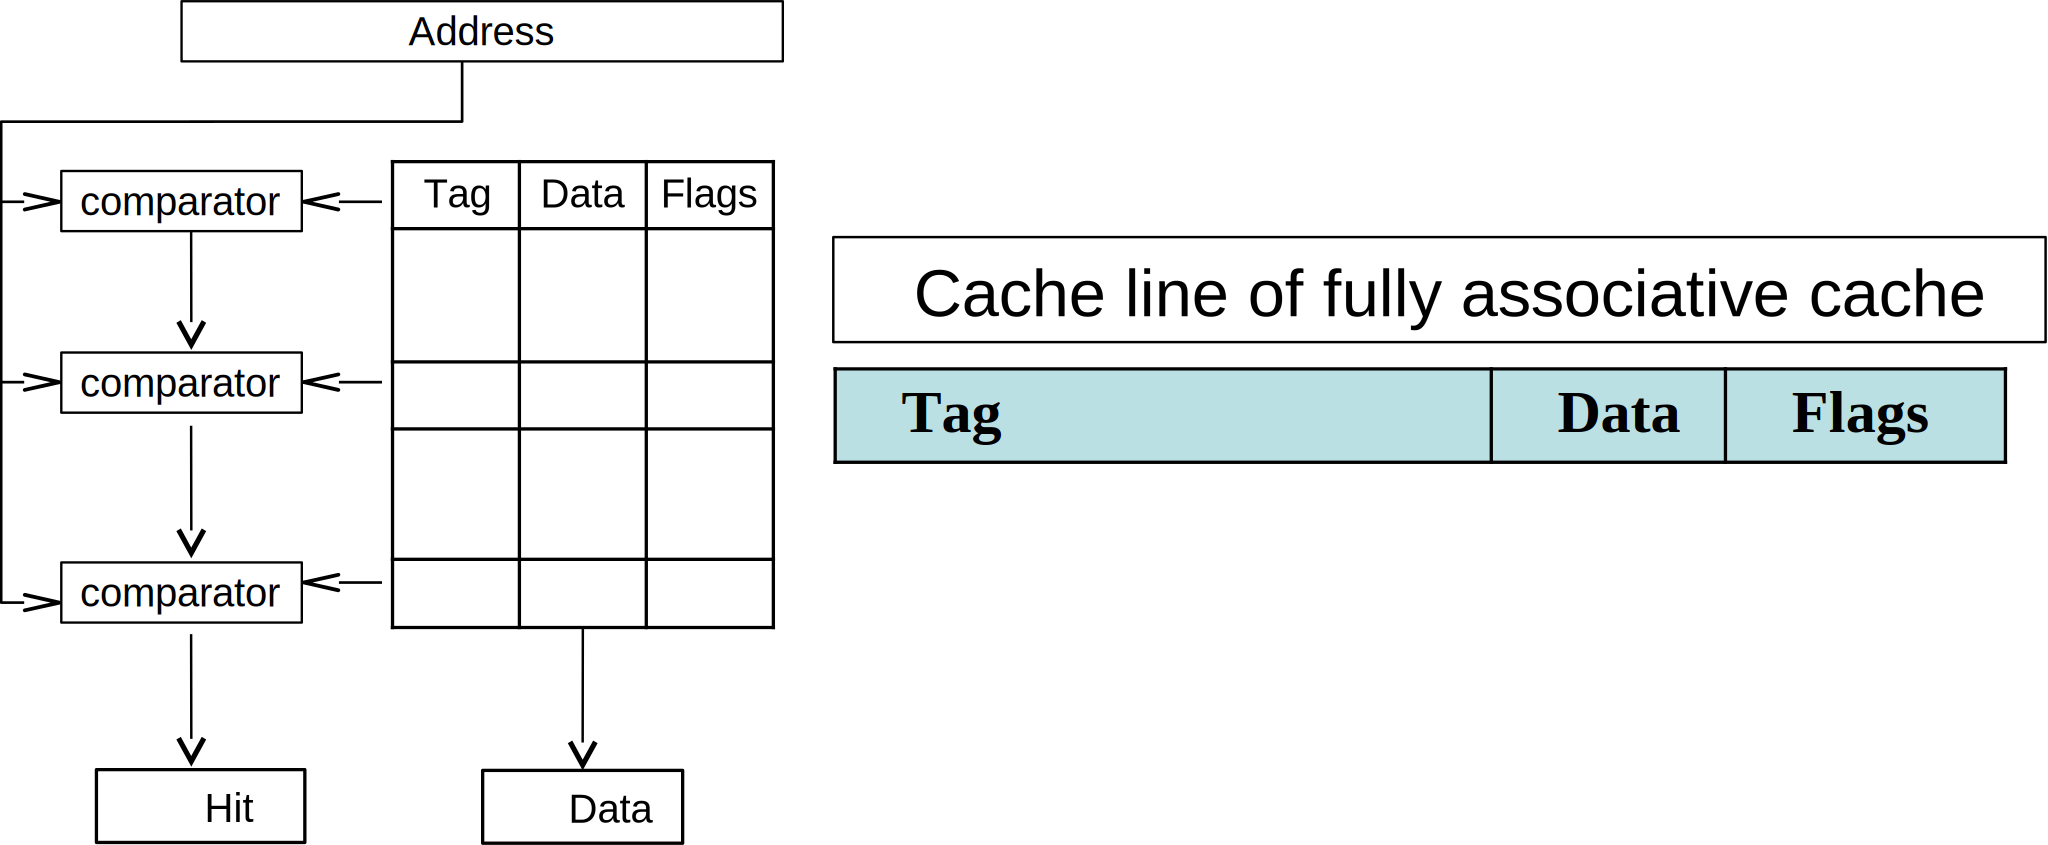
\includegraphics[width=0.70\linewidth]{cache-principle.pdf}

}
\vskip 2mm

\begin{itemize}
\item \textbf{Tag} je index odpovídajícího bloku v operační paměti (v podstatě se jedná o hodnotu ukazatele/adresy dělenou délkou bloku).
\item \textbf{Data} pole obsahující vlastní hodnoty na příslušné/ných adrese/ách.
\item \textbf{Validity bit} – bit platnosti. Indikuje, zda je obsah pole Data vůbec platný.  
\item \textbf{Dirty bit} – rozšiřující pole v obsahu paměti. Indikuje, že v cache (cache) je jiná hodnota, než v paměti hlavní.
\end{itemize}

\end{frame}


\begin{frame}
\frametitle{Zpracování výpadku skryté paměti, cache miss}

\begin{itemize}
\item Data musí být nahrána z hlavní paměti, obvykle jsou již ale všechny položky vyrovnávací paměťi (cache) zaplněné daty z přetrvávajícími předchozího běhu programu.
\item Některou z položek, kterou je možné využít pro uložení dat z dané adresy je potřeba uvolnit.
\item Na výběru položky k vyřazení velmi záleží, pokud bude vybraná ta, která bude opětovně potřeba, dojde k snížení výkonu.
\item \textbf{Cache replacement policy} -- pravidla pro výběr položky k vyřazení
\begin{itemize}
\item \textbf{Random} -- vybraná je náhodná položka
\item \textbf{LRU} (Least Recently Used) -- vybrána je nejdelší dobu neoužitá položka, do obvodů cache musí být ke každé skupině bloků přidané další informace, které umožňují sledovat pořadí posledních přístupů k jednotlivým položkám.
\item \textbf{LFU} (Least Frequently Used) -- sleduje se, jak často/kolikrát se k položkám přistupuje, vyžaduje přidat zapomínání.
\item \textbf{ARC} (Adaptive Replacement Cache) – kombinace LRU a LFU
\end{itemize}
\end{itemize}

\end{frame}

\begin{frame}
\frametitle{Zápisy procesoru do hlavní paměti}

\begin{itemize}
\item V cestě je cache, která může blok, do kterého je zapisováno, obsahovat.
\item Minimálně z pohledu daného procesoru je nutné zajistit koherenci dat pro daný procesor (často i pro více procesorů -- vlákna) pro přístupy ke každé jednotlivé adrese i pokud existuje více cest přístupu 
\item \textbf{Write through} (zápis, propsání zkrz) cache -- pokud se již data v cache nahází jsou modifikovaná, ve variantě s automatickou alokací jsou i při výpadku nahraná a pak modifikovaná. Data jsou zároveň odeslaná do hlavní paměti, buď přímo nebo přes zápisovou frrontu (write buffer)
\item \textbf{Write back} -- data jsou zapsaná do příslušného bloku cache, pokud není v cache, je blok nejdříve načtený. Blok je označený \textbf{dirty bit}em. Zápis do další úrovně až pokdu je potřeba danou položku cache umolnit pro jiná data (replacement) nebo je vyžádaná sychronizace procesorem, systémem (cache flush).
\end{itemize}

\end{frame}

\begin{frame}
\frametitle{Základní typy organizace paměti cache}

Uvažujeme cache o velikosti 8 bloků a kam může být mapovaný přístup na adresu/blok 12 pro tři varianty organizace skryté paměti

\begin{tabular}{p{0.29\linewidth}p{0.29\linewidth}p{0.29\linewidth}}
\textbf{Plně asociativní} & \textbf{Přímo mapovaná} & \textbf{Dvoucestná} \\
\textbf{Fully associative:} & \textbf{Direct mapped} & \textbf{2-way associative} \\
Adresa 12 může být umístěna libovolně &
Adresa 12 může být umístěna jen do bloku 4 (12 mod 8) &
Adresa 12 může být umístěna do sady 0 (12 mod 4) \\
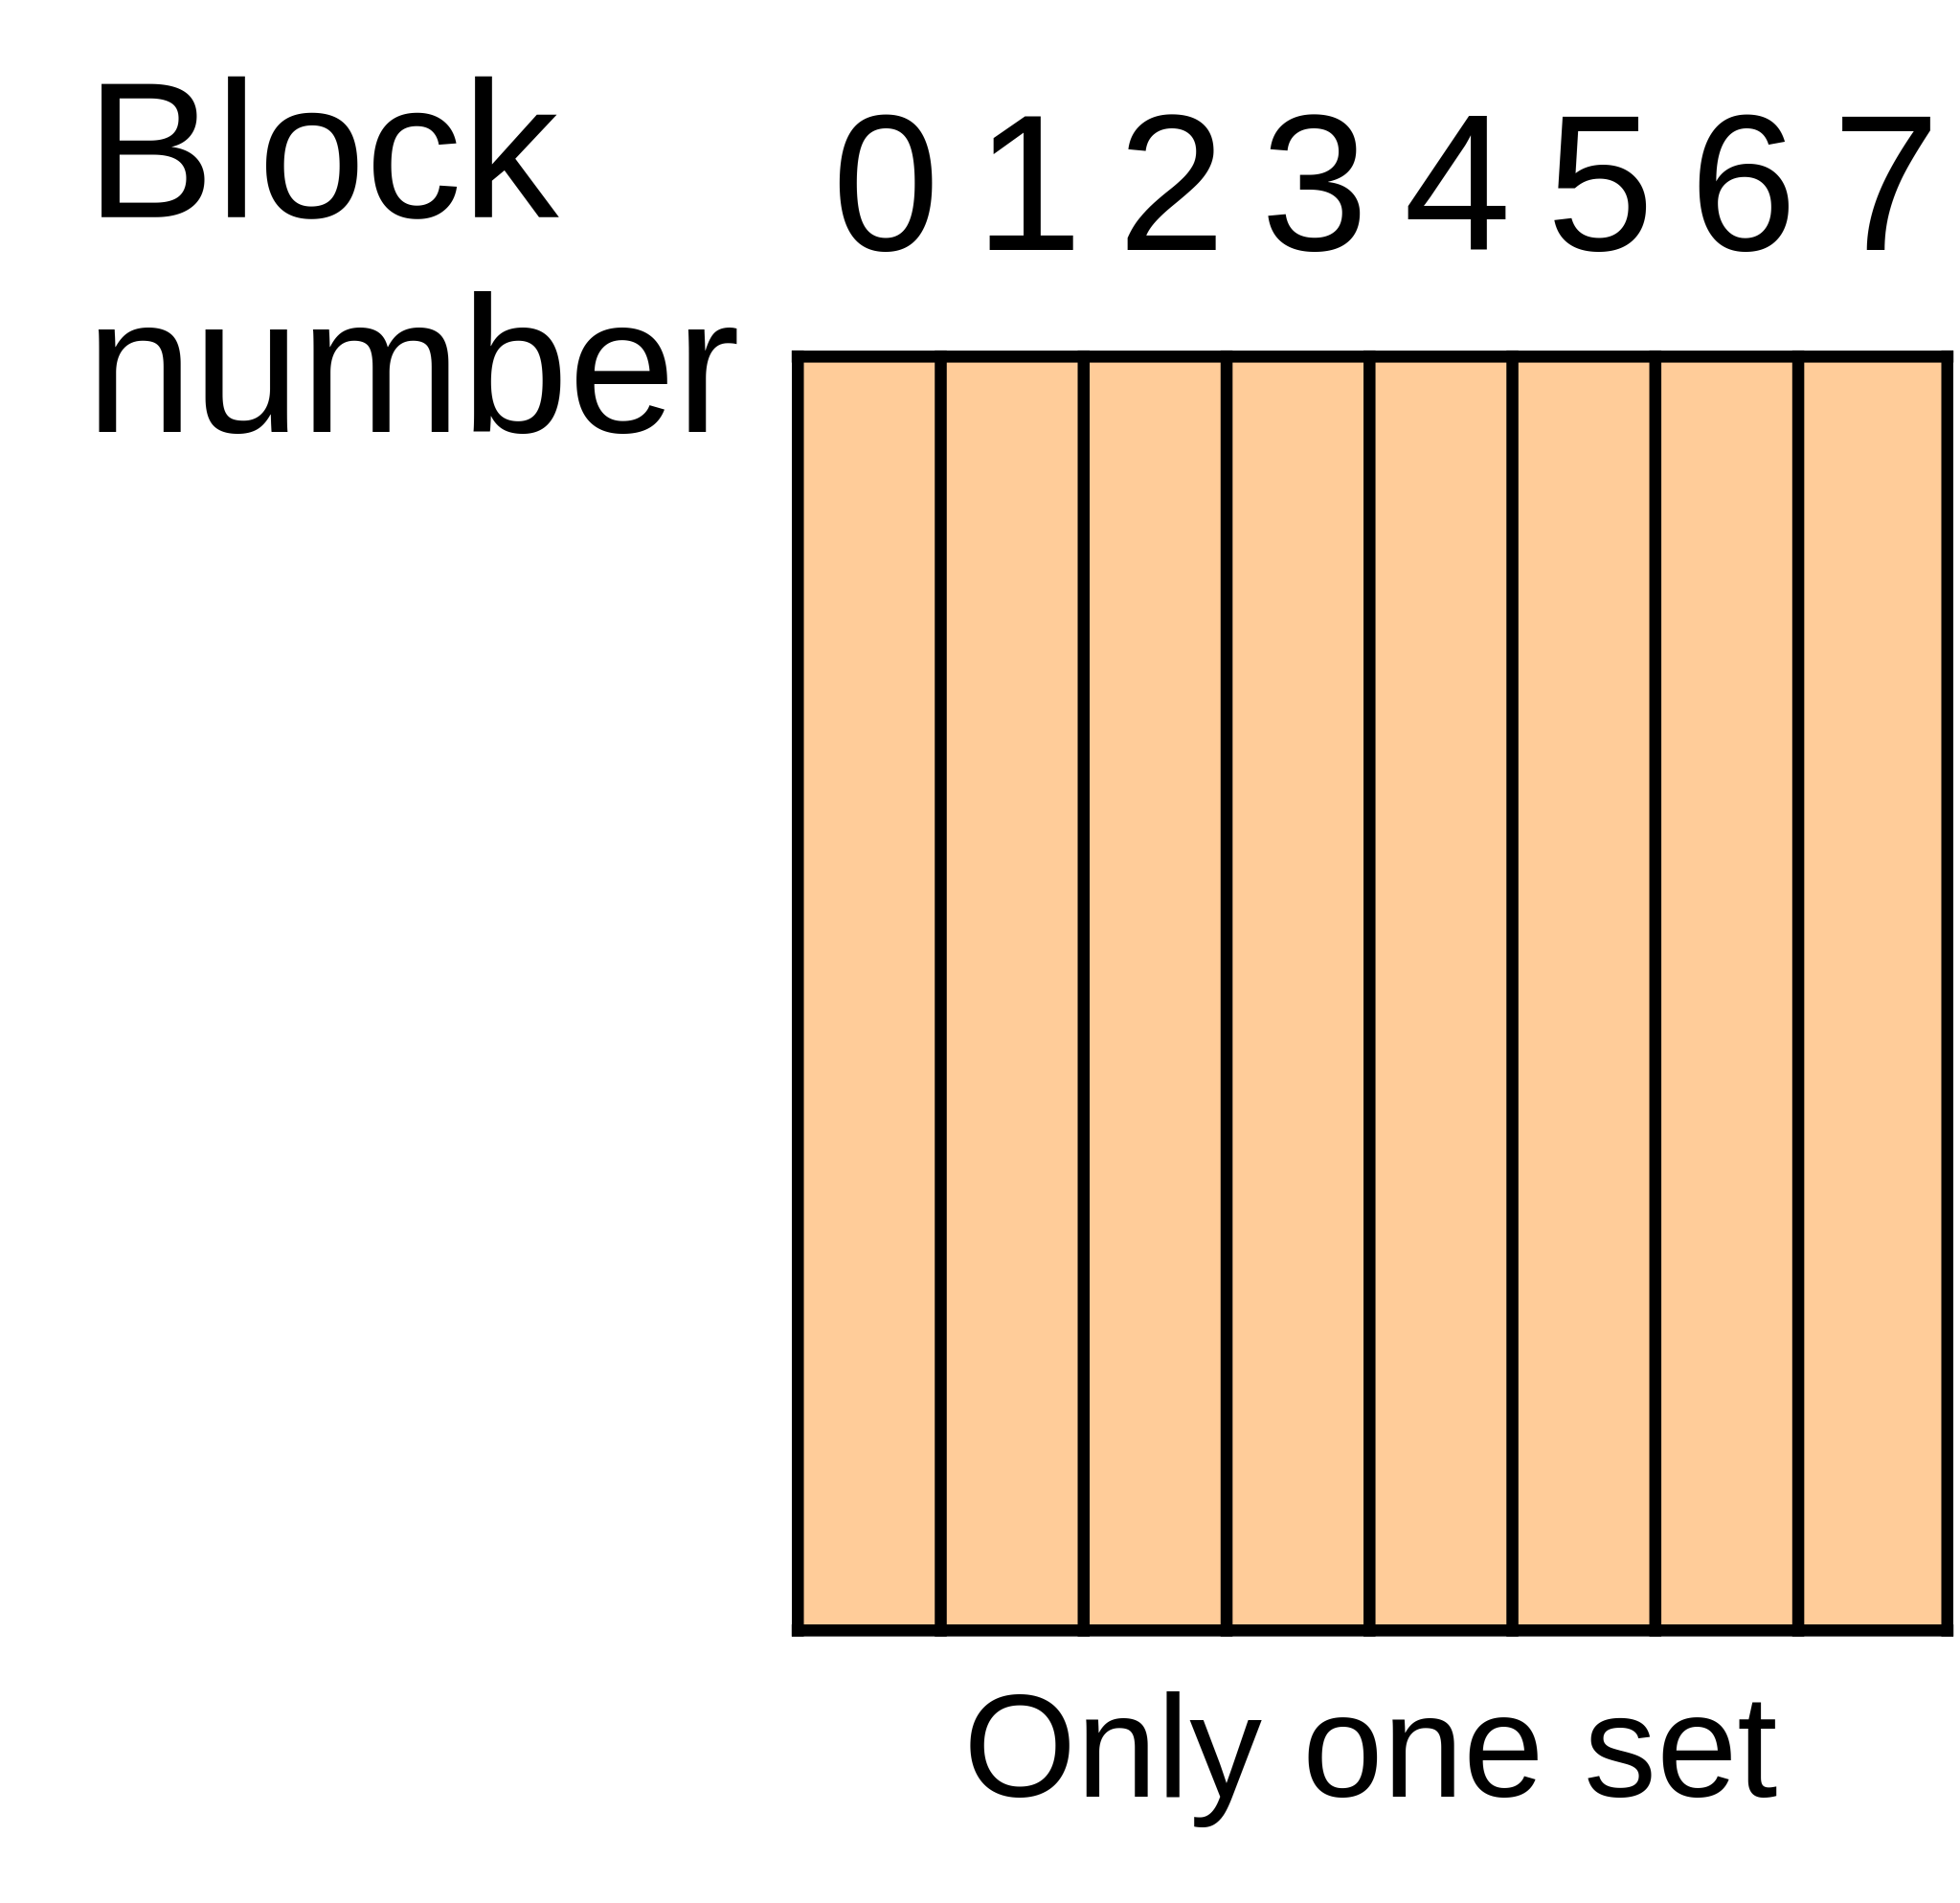
\includegraphics[width=3cm]{cache-schema-fully.pdf} &
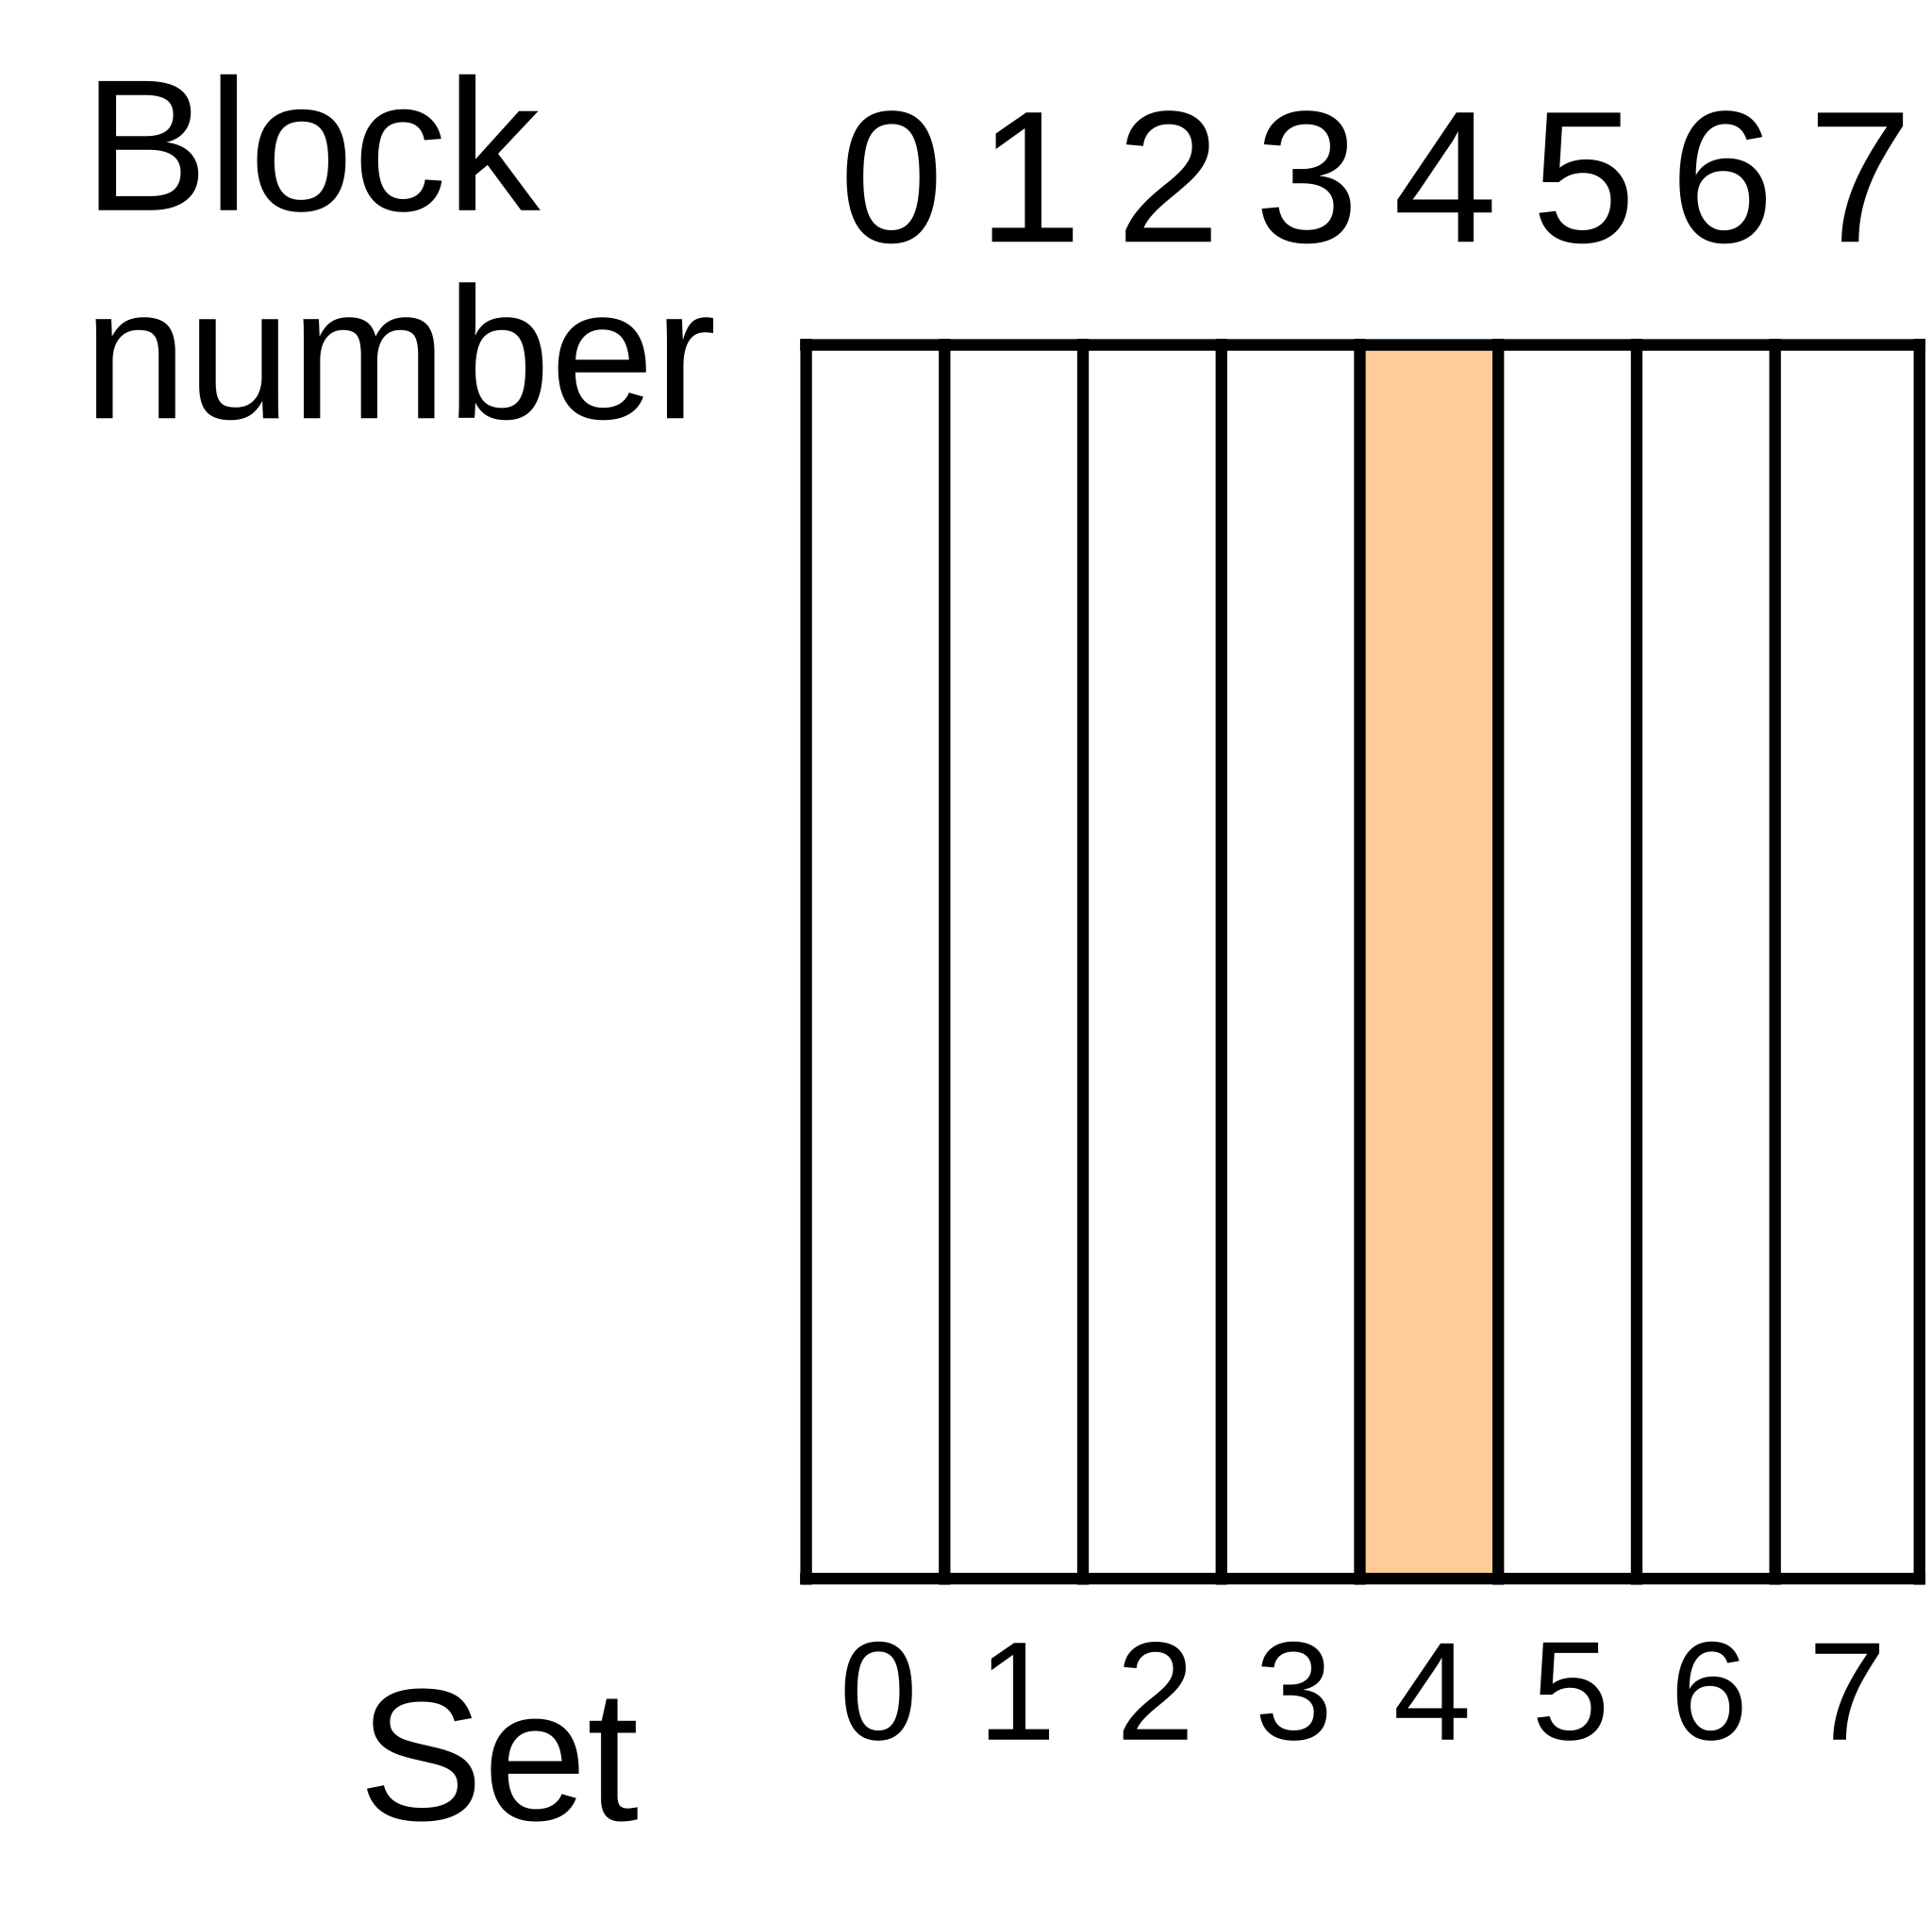
\includegraphics[width=3cm]{cache-schema-direct.pdf} &
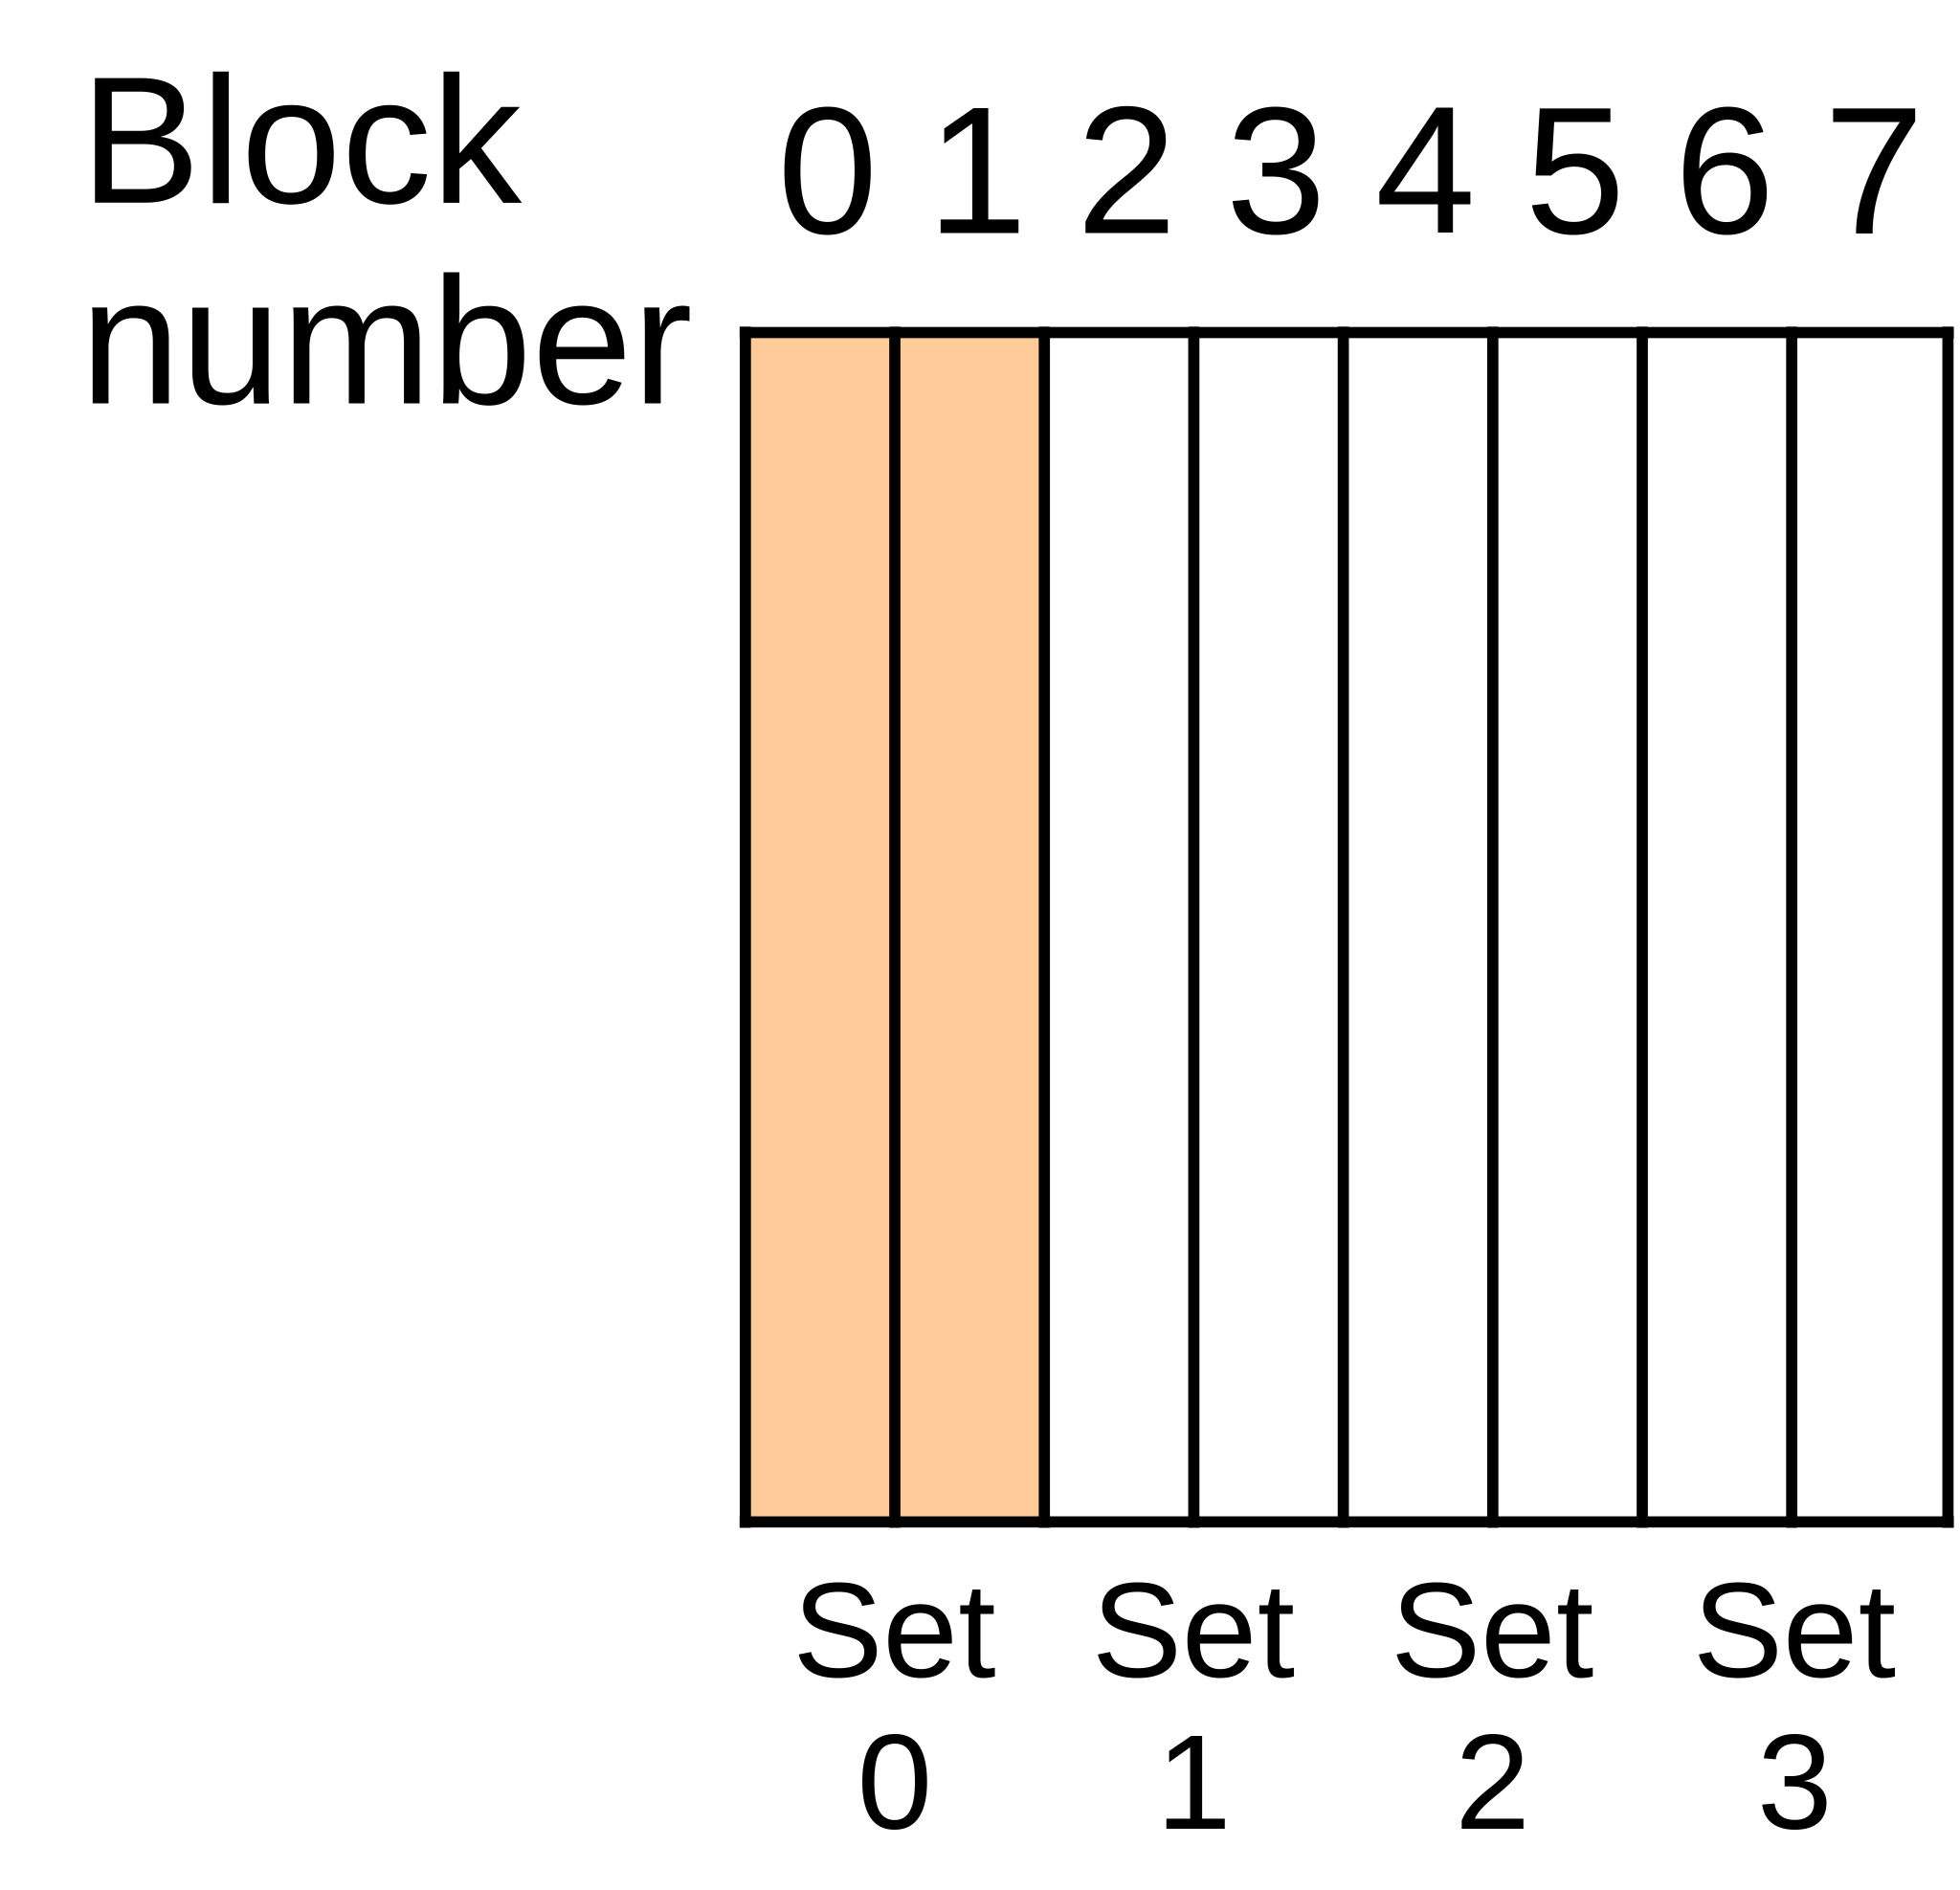
\includegraphics[width=3cm]{cache-schema-2way.pdf} \\
\end{tabular}

\end{frame}

\begin{frame}
\frametitle{Přímo mapovaná paměť cache -- mapování}

{
\centering

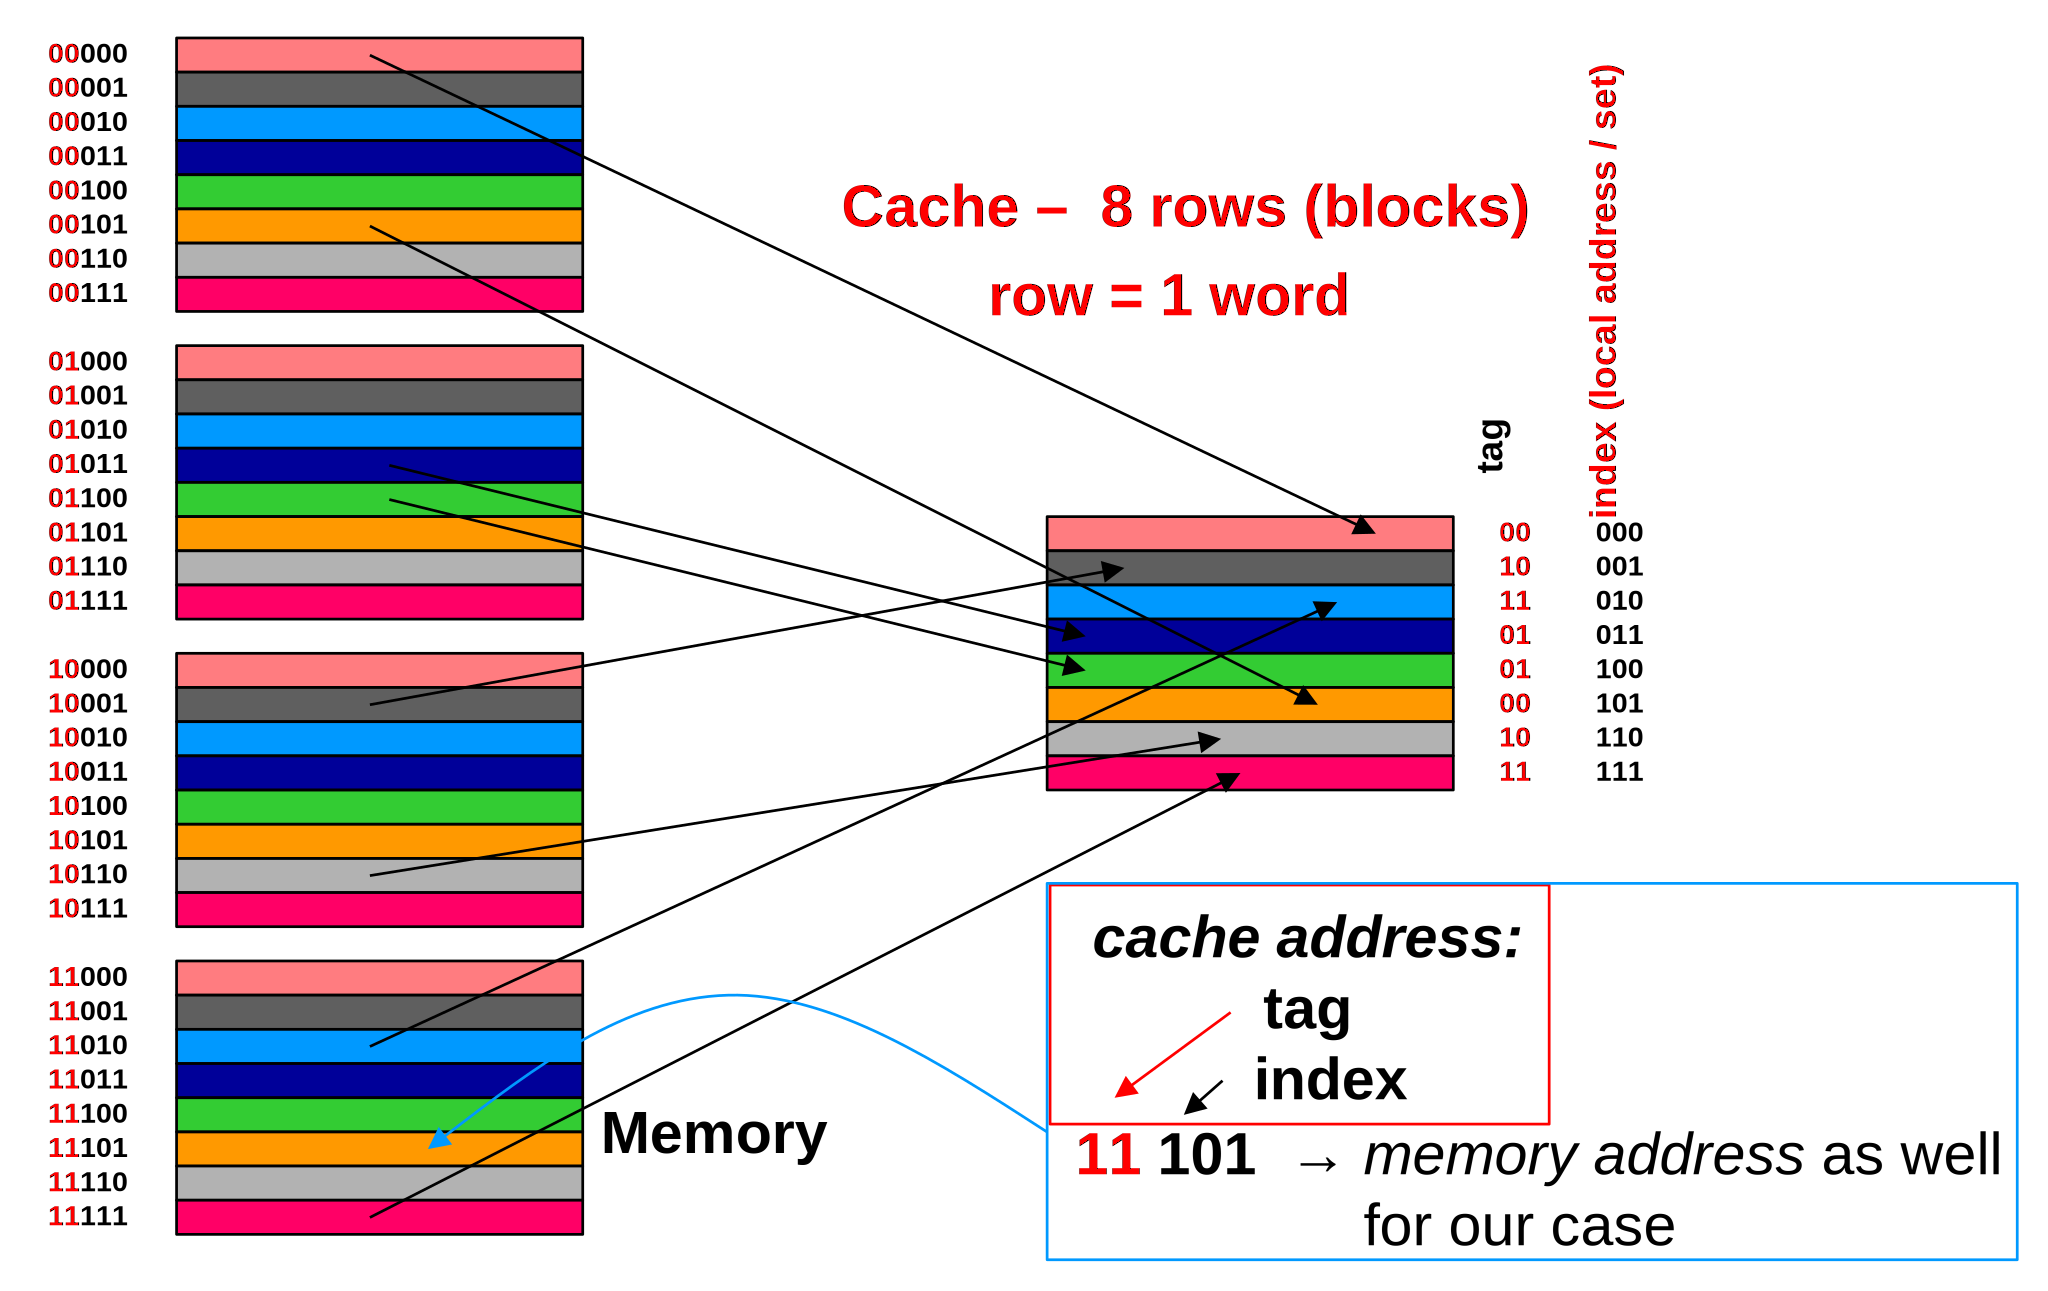
\includegraphics[width=0.9\linewidth]{cache-direct-mapping-1byte.pdf}

}

\end{frame}

\begin{frame}
\frametitle{Přímo mapovaná paměť cache s blokem rovným slovu}

\begin{itemize}
\item \textbf{Capacity} -- C ... kapacita (zde 1024 v bytech a 256 v slovech)
\item \textbf{Number of sets} -- SN .. počet setů, (zde 256)
\item \textbf{Word size} – WS .. velikost bloku (zde 4 byte)
\item \textbf{Block size} – BS .. velikost bloku (zde 1 slovo, 4 byte)
\item \textbf{Number of blocks} -- BN .. počet bloků (zde 256)
\item \textbf{Degree of associativity} -- N . stupeň asciativity, počet cest (zde 1)
\end{itemize}

{
\centering

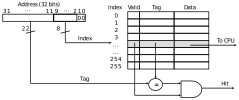
\includegraphics[width=0.70\linewidth]{cache-direct-simple.pdf}

}

C = 1024 bytů, SN = BN = 256, BS = 1, N = 1

\end{frame}


\begin{frame}
\frametitle{Přímomapovaná paměť cache s většími bloky}

BS = 4 (16 byte, slovo WS = 4 byte), setů SN = 4

set = (adresa div BS) mod SN

{
\centering

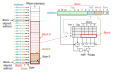
\includegraphics[width=0.75\linewidth]{cache-direct-ms.pdf}

}

{\tiny Zdroj: Michal Štepanovský}
\end{frame}

\begin{frame}
\frametitle{Obecná organizace paměti cache s N cestami}

{
\centering

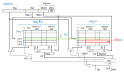
\includegraphics[width=0.95\linewidth]{cache-n-way-ms.pdf}

}

{\tiny Zdroj: Michal Štepanovský}

\end{frame}

\begin{frame}
\frametitle{Ukázka: QtRvSim vect-inc, vect-add2, vect-add}

\end{frame}

\begin{frame}
\frametitle{Vliv velikosti a organizace cache na počty výpadků}

{
\centering

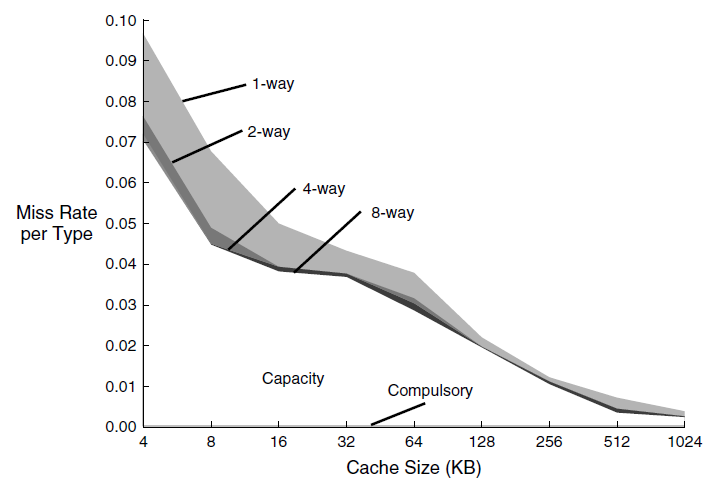
\includegraphics[width=0.65\linewidth]{fig/cache-size-vs-ways.png}

}

\begin{itemize}
\item miss rate není vlastnost, parameter cache
\item miss rate není vlastnost programu
\end{itemize}

Jedná se o kombinaci jak algoritmů v programu, tak parametrů cache a často i zpracovávaných dat.

\end{frame}

\begin{frame}
\frametitle{Vliv velikosti bloku a celé cache na počty výpadků}

{
\centering

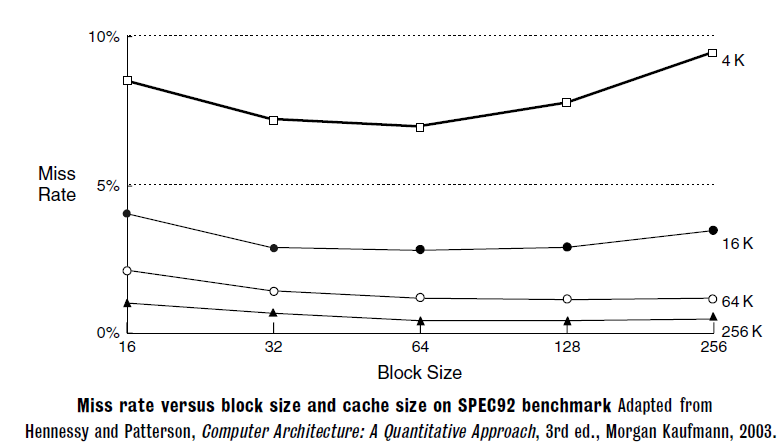
\includegraphics[width=0.75\linewidth]{fig/cache-size-vs-block.png}

}

Zvětšení velikosti bloku napomáhá načtení sousedních dat, která mohou být často následně potřeba.
Ale pokud tomu tak není, tak se zvyšuje cache miss penalty a zároveň dochází častěji ke kolizím
a obsazení cache nepotřebnými daty.

\end{frame}

\section{Virtuální paměť a stránkování}

\begin{frame}
\frametitle{Paměťové prostory procesů a odkládání na disk}

Více procesů, každý vlastní paměťový prostor. Vzájemná ochrana
a možnost rozšíření kapacity hlavní paměti o prostor na sekundární -- swap.

{
\centering

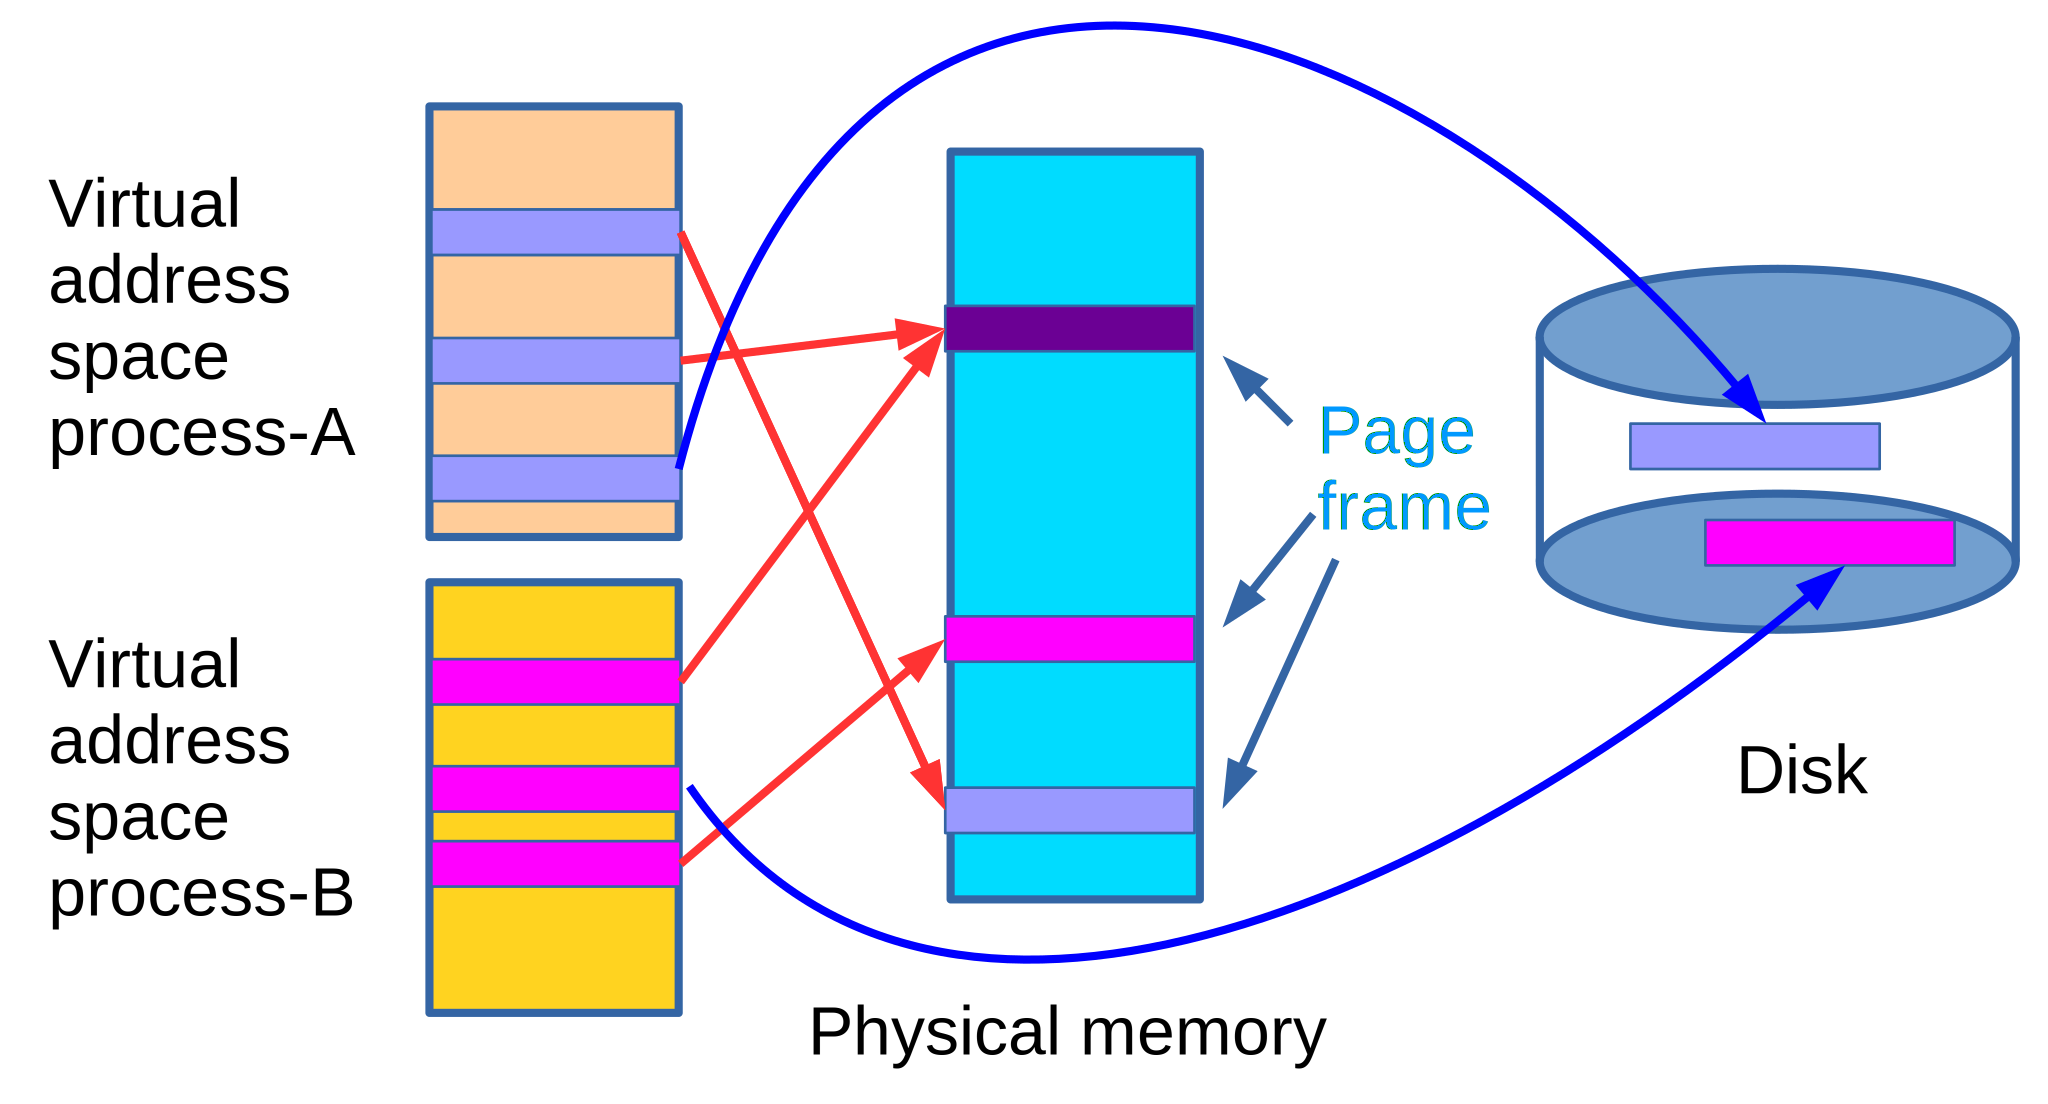
\includegraphics[width=0.80\linewidth]{paging-to-disc.pdf}

}

Překlad po jednotlivých bytech by byl drahý, prostor je rozdělěný na~stránky
(zarovnané), typicky 4\,kB, někdy i větší, např. 64\,kB.

\end{frame}

\begin{frame}
\frametitle{Překlad virtuální a fyzické adresy}

Překlad překlad zajišťuje \textbf{Memory Management Unit} (MMU).

Pro po vyplnění stránkovacích tabulek a nastavení \textbf{Page Directory Base Register}
(PDBR) operačním systémem probíhá překlad na stránky přítomné v paměti většinou automaticky.

Naopak výpadky stránek ošetřují rutiny operačního systému. Pokud je přístup do namapované
oblasti, načtou data z disku, sítě, odkládacího oddílu.

Stějně jako u cache je zde nutné a náročné hledat prostor pro nově potřebné stránky (princip podobný LRU).

\vskip 2mm

{
\centering

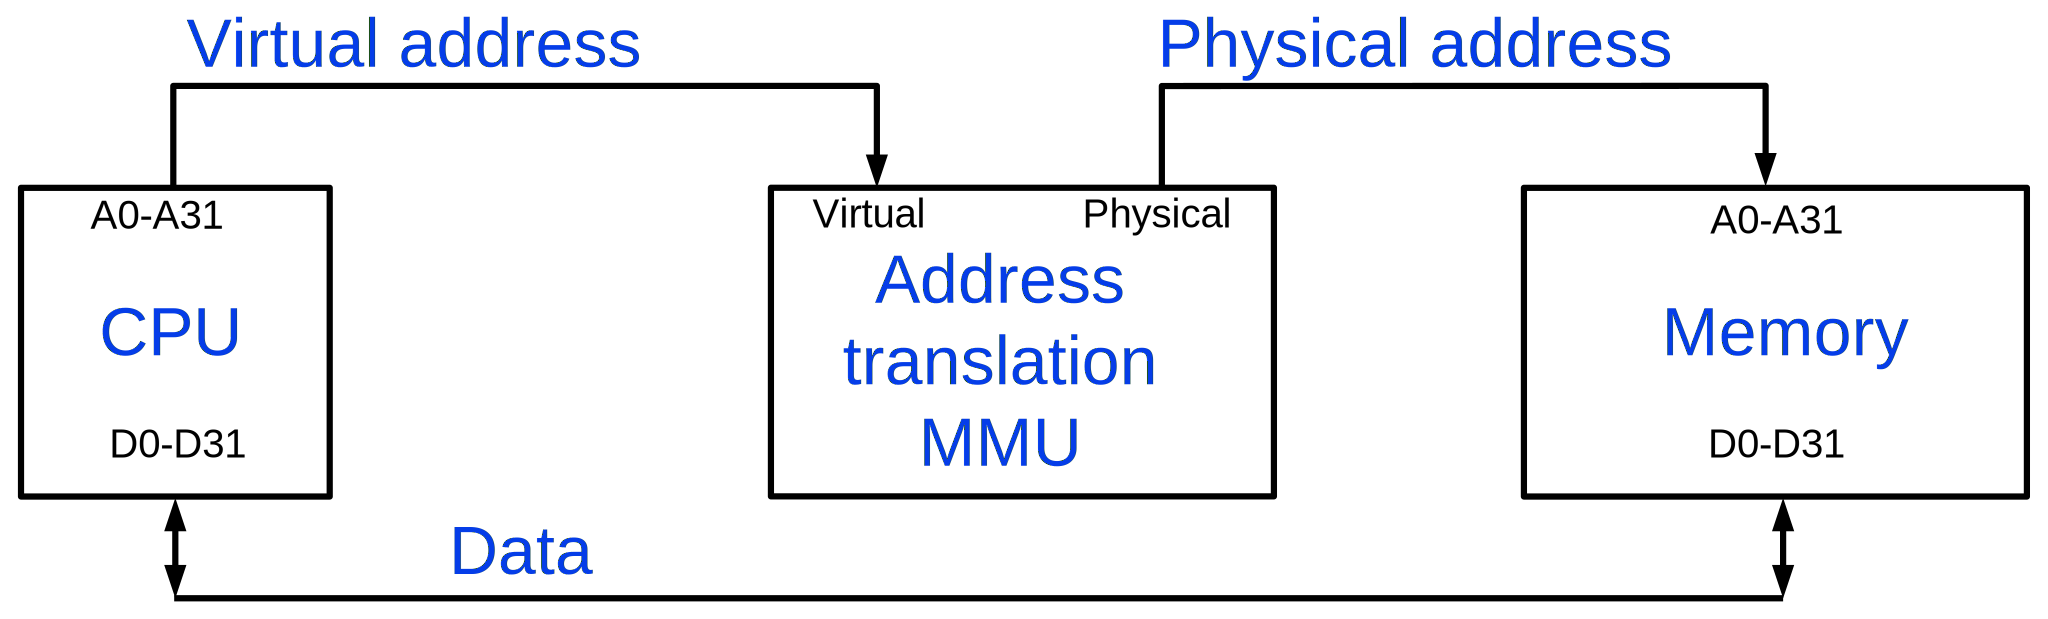
\includegraphics[width=0.80\linewidth]{paging-cpu-mm-mem.pdf}

}
\end{frame}

\begin{frame}
\frametitle{Jednoúrovňová stránkovací tabulka}

{
\centering

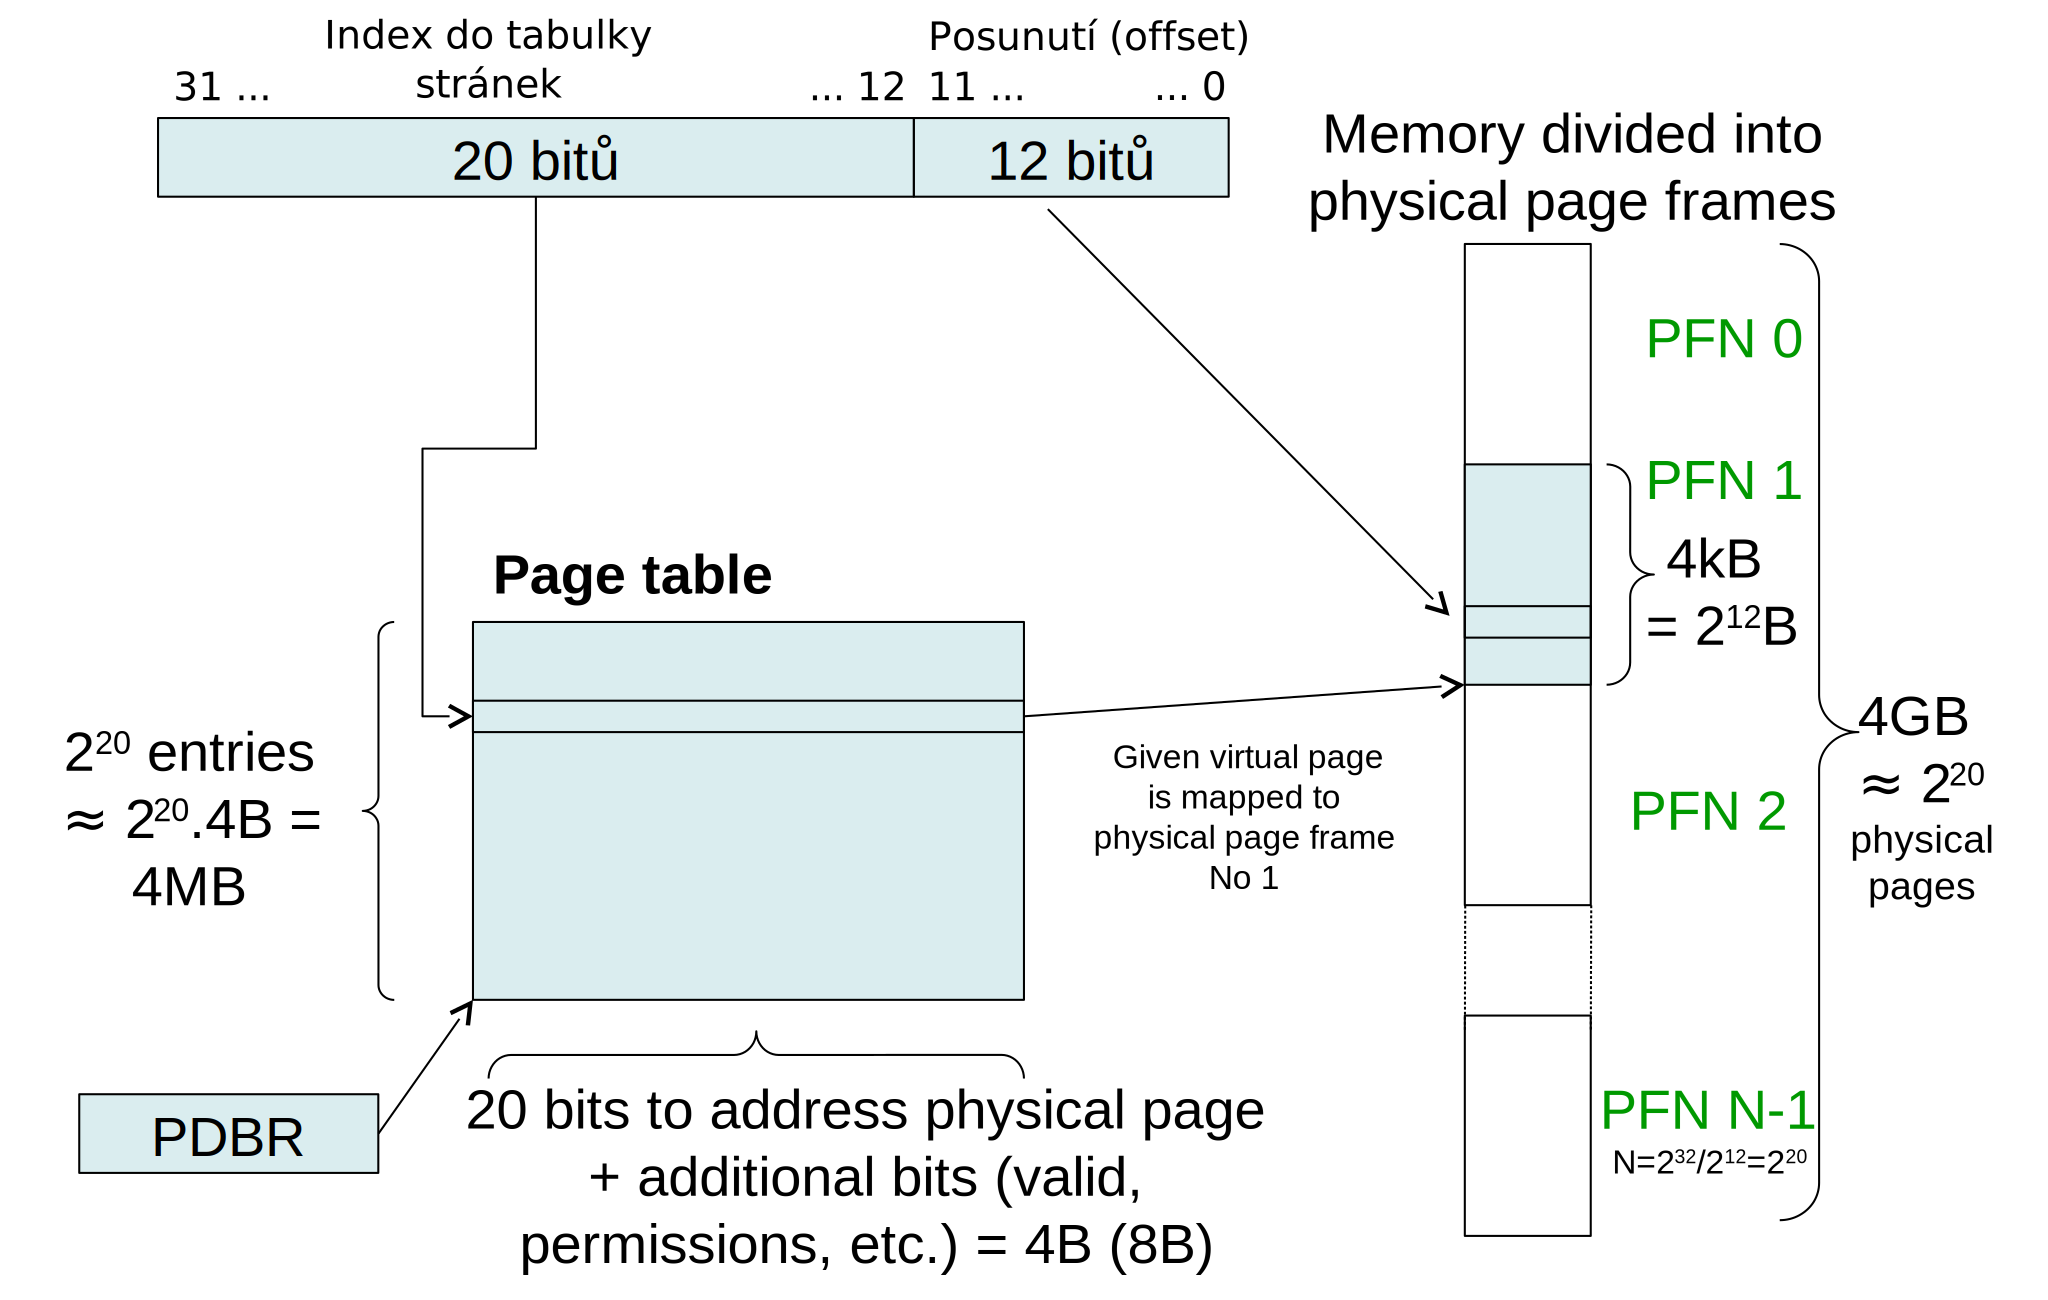
\includegraphics[width=0.80\linewidth]{paging-1-level.pdf}

}

Řešení je nevýhodné, pro každý, i malý, spuštěný proces je na 32-bitovém
systému pro 4\,kB stránky potřeba alokovat 4\,MB (překlad 20-bitů adresy,
4-byte na 32-bit položku) 

\end{frame}


\begin{frame}
\frametitle{Dvouúrovňové stránkování}

{
\centering

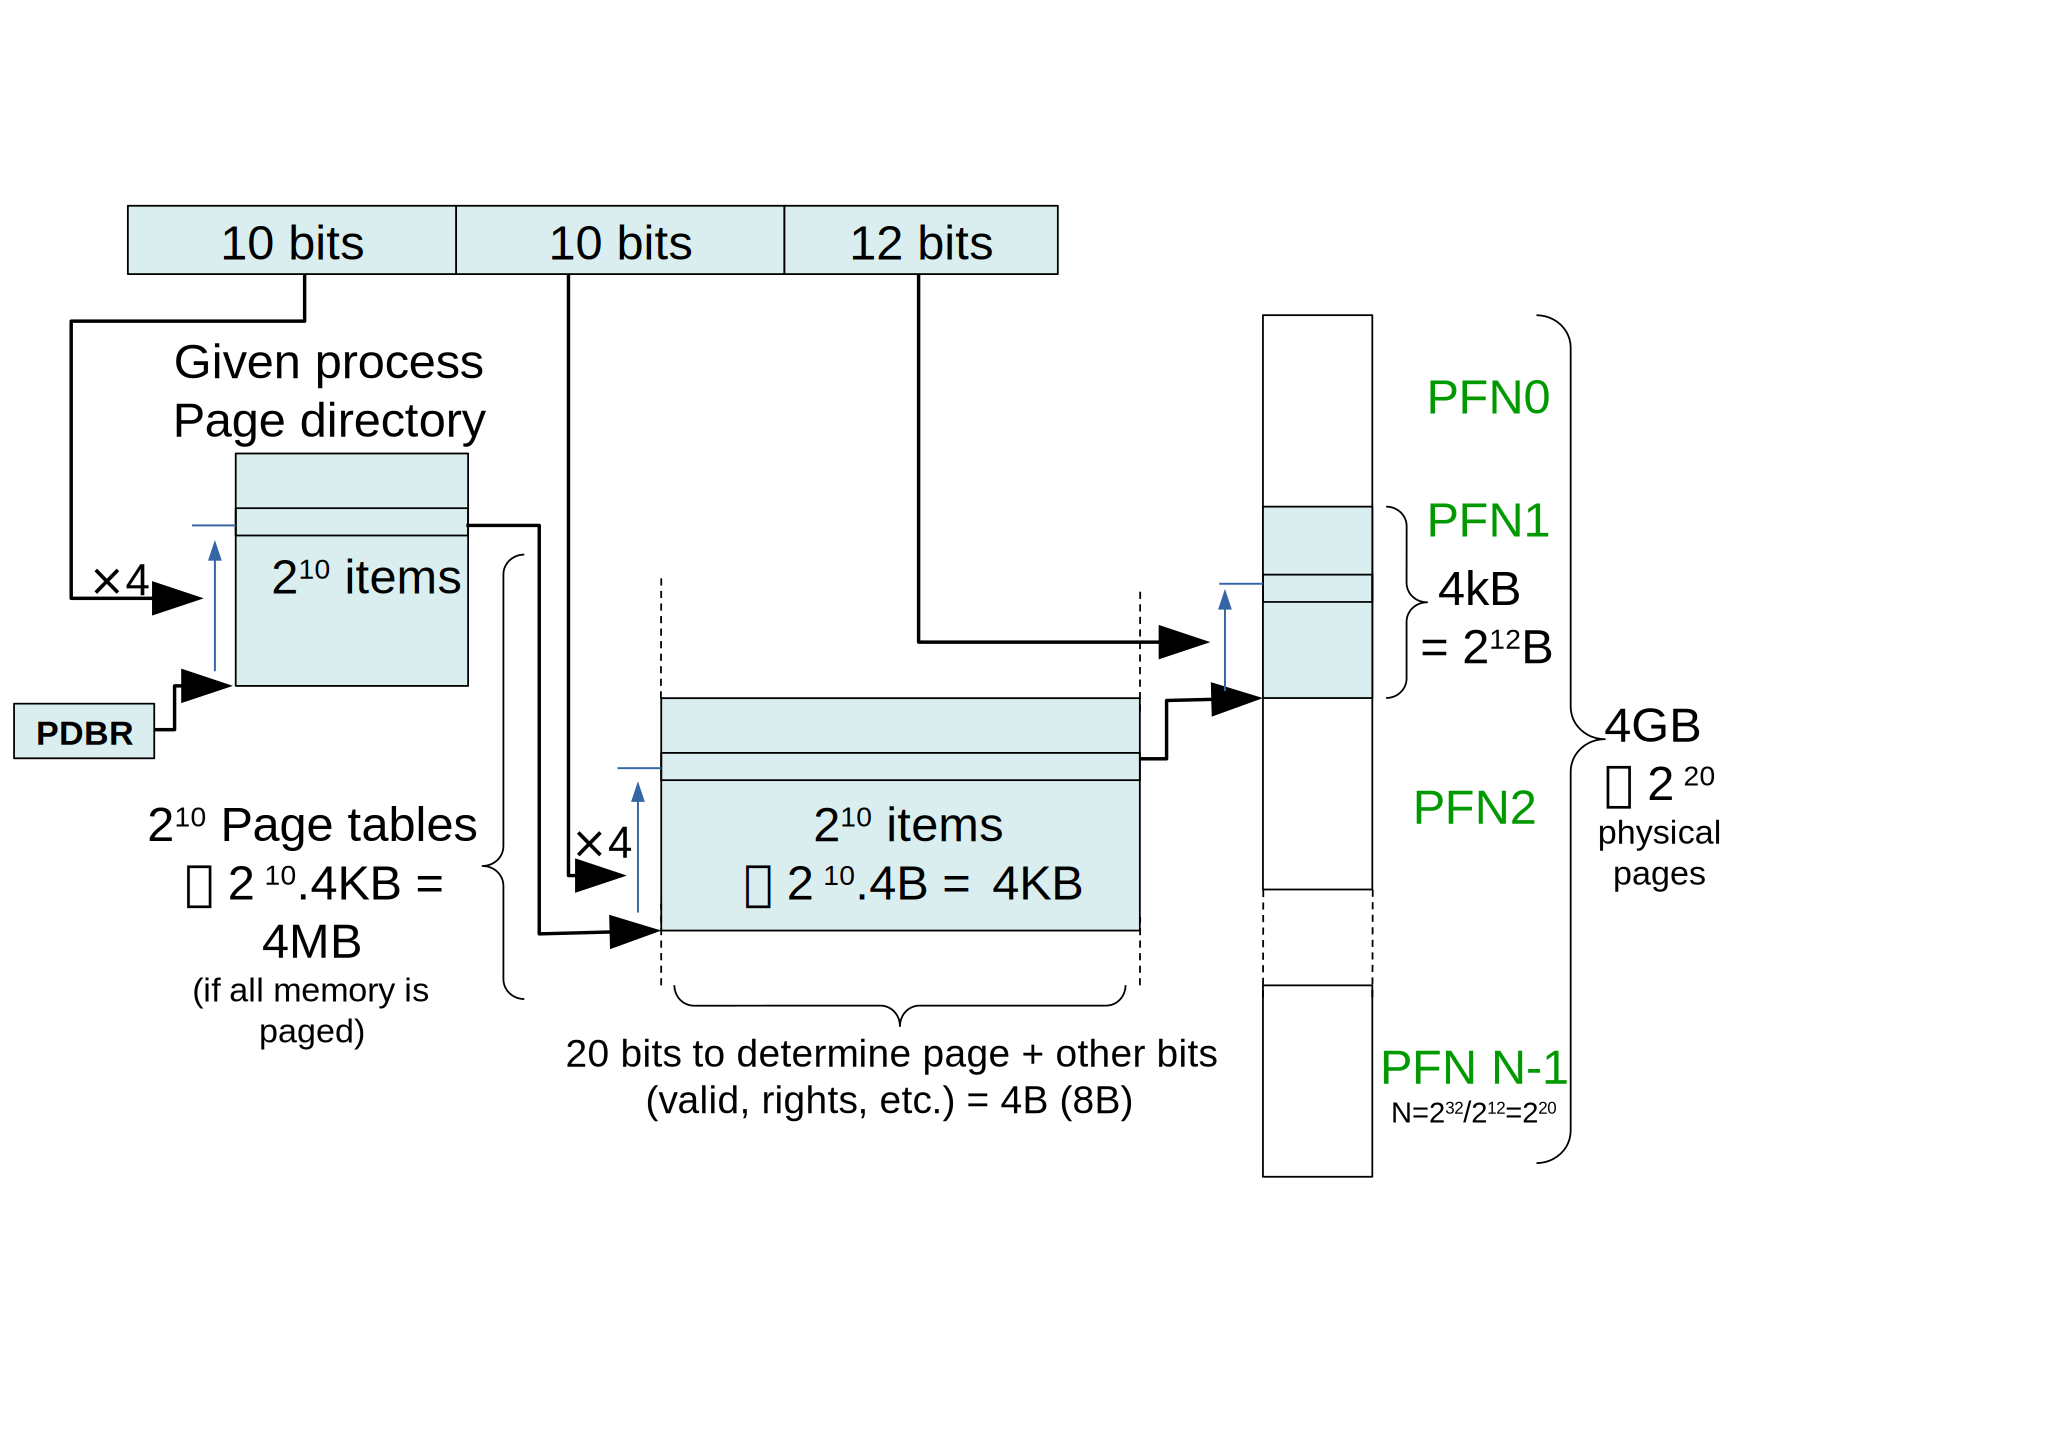
\includegraphics[width=0.75\linewidth]{paging-2-levels.pdf}

}

Adresář stránek pro každý proces, úroveň tabulek s vlastními položekami
se alokuje jen, když je daná oblast virtuálního prostoru použitá.

Za pozornost stojí, že při překladu po 10-ti bitech vychází pole položek
adresáře i tabulky na velikost 4\,kB. Nepotřebuje aloace vyššího řádu
ohrožené fragmentací.

\end{frame}

\begin{frame}
\frametitle{Položky adresářů stránek -- \textbf{Page Directory Entry} (PDE) }

{
\centering

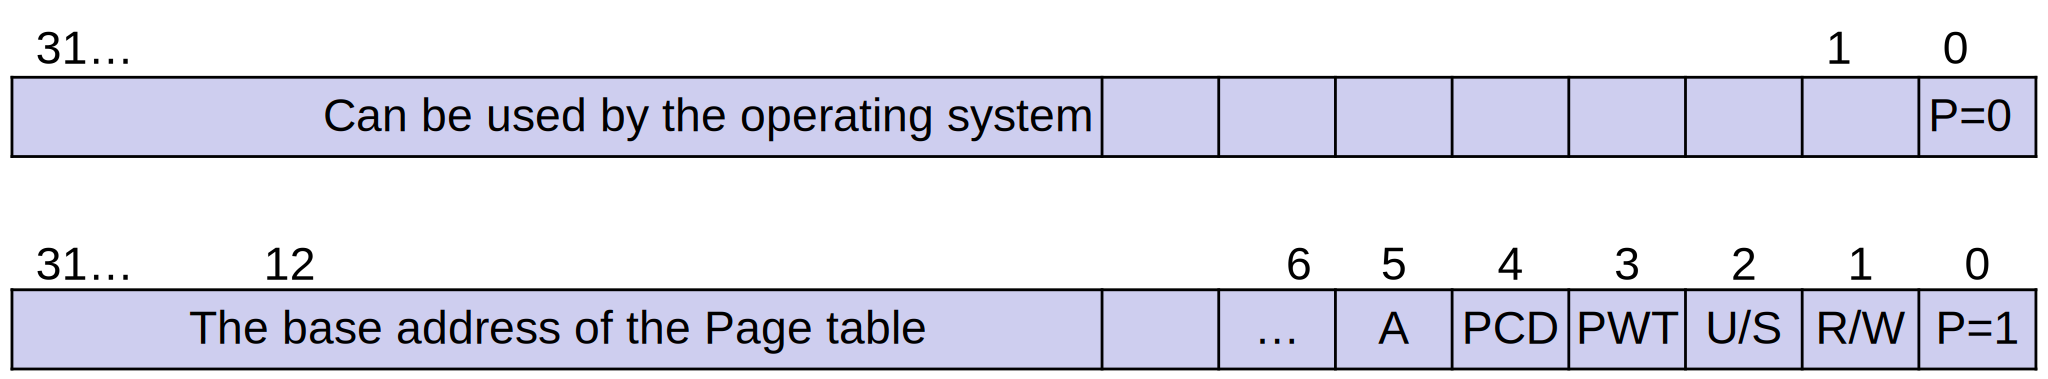
\includegraphics[width=0.90\linewidth]{paging-pde-1.pdf}

}

\vskip 2mm

\begin{itemize}
\item bit 0: Present bit -- další úroveň nebo stránka je přítomná v paměti (1). Pokud není (0) tak jsou data uložena na disku nebo oblast není mapovaná. Někdy také bit označovaný V -- valid bit.
\item bit 1: Read/Write: 1 -- R/W -- zápis povolený; 0 -- read only (RO)
\item bit 2: User/Supervisor: 1 -- přístupné uživateli; 0 -- přístup jen operační systém
\item bit 3: Write-through/Write-back -- nastavení typu přístupu
\item bit 4: Cache disabled/enabled -- důležité pro paměťově mapované periferie, přímý přístup do registrů bez cache
\item bit 5: Accessed -- nastaven MMU při prvním přístupu z procesoru
\end{itemize}

\end{frame}

\begin{frame}
\frametitle{Položky koncových tabulek -- \textbf{Page Table Entry} (PTE)}

{
\centering

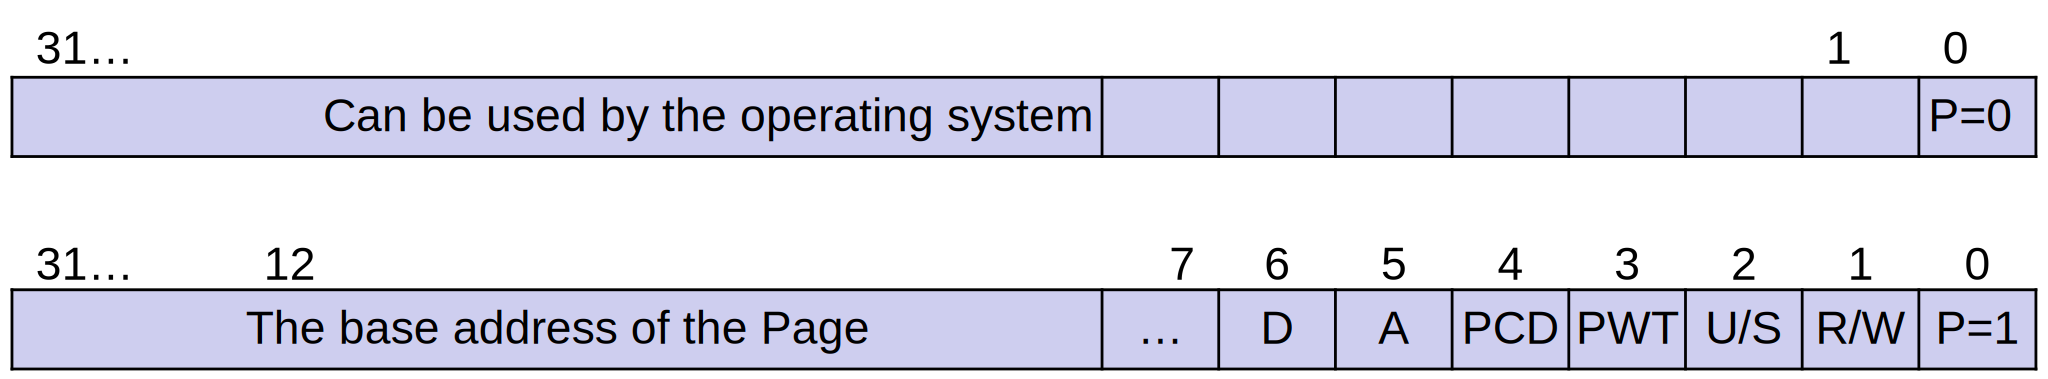
\includegraphics[width=0.90\linewidth]{paging-pte.pdf}

}

\vskip 2mm

\begin{itemize}
\item bit 6: Dirty bit, případně někdy Modified – jen nastavený MMU, pokud došlo k zápisu do dané stránky od poslední kontroly a případného nulování příznaku operačním systémem.
\item Ostatní bity mají stejný význam jako v položce adresáře
\end{itemize}

Bit \textbf{Accessed} je klíčový, když operační systém hledá stránky fyzické paměti k uvolnění.
Obvykle počítá podle bitů další, obsáhlejší, statistiku a při průchodu seznamem bity nuluje.
Pokud je nastavený \textbf{Dirty}, tak je při uvolnění fyzciké stránky (PFN) je nutné data
sychronizovat zpět do~souboru, odkládacího oddílu atd.

\end{frame}


\begin{frame}
\frametitle{Překlad na 64-bitových architekturách}

{
\centering

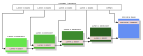
\includegraphics[width=0.90\linewidth]{address-trans-4-levels.pdf}

}

Vyžaduje více úrovní. Pro 64-bitů a 4\,kB stránky je teoreticky
potřeba přeložit 52-bitů. Pokud jednotlivé části tabulek mají
zaplnit jednu stránku, tak vychází překlad na 9\,bitů ($512 \times 8 = 4096$)
na úroveň a tedy $ceil(52 / 9) = 6$. Často se ale jedna až dvě úrovně vynechávají, více později.


\end{frame}

\begin{frame}
\frametitle{Zrychlení opakovaného překladu}

Každý překlad představuje několik přístupů do~paměti a i když je urychlený
přístupy přes cache, tak zpomaluje. Zavádí se \textbf{Translation Look-Aside Buffer} (TLB).
Pracuje na shodném principu jako paměťová cache, ale ukládá k virtuální adrese
její překlad na~fyzickou. Opět omezená kapacita, LRU a~nutnost brát v~potaz
při~programování.

\vskip 2mm

{
\centering

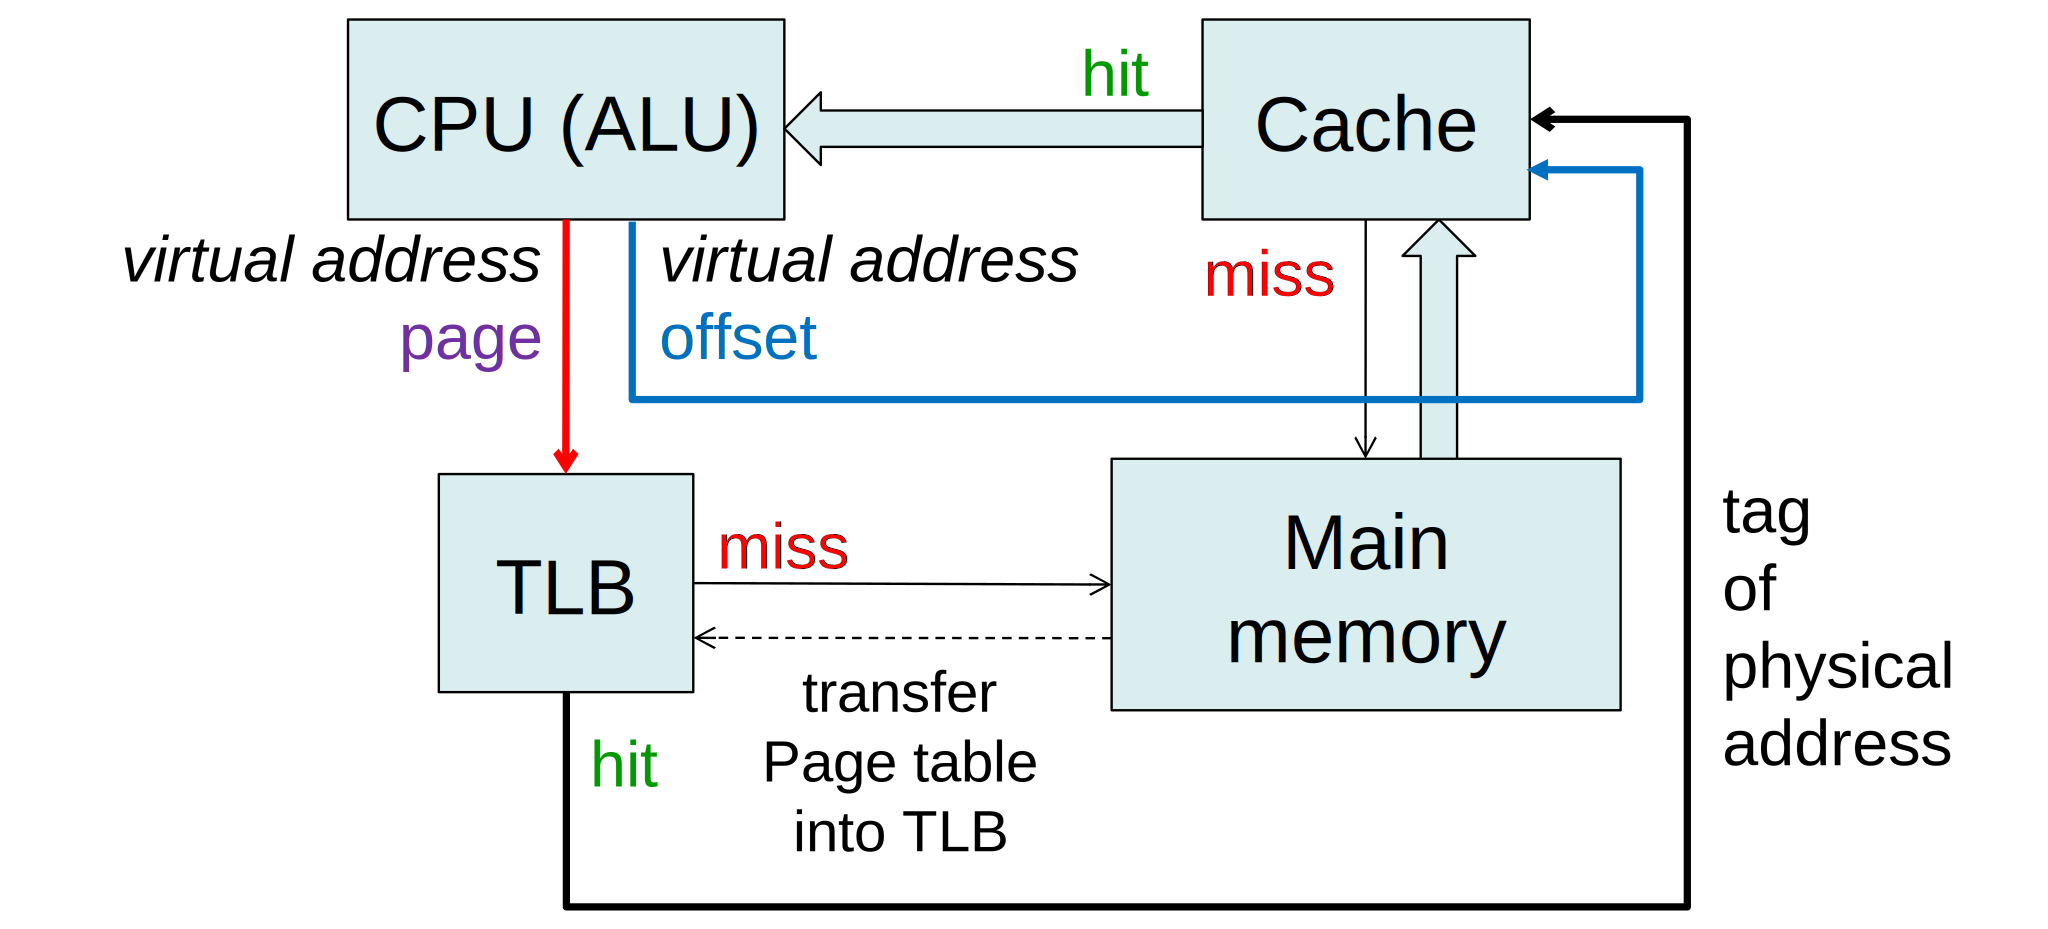
\includegraphics[width=0.80\linewidth]{paging-tlb.pdf}

}
\end{frame}

\section{Cache a stránkování dohromady}

\begin{frame}
\frametitle{Paměťový subystém - Intel Nehalem}

{
\centering

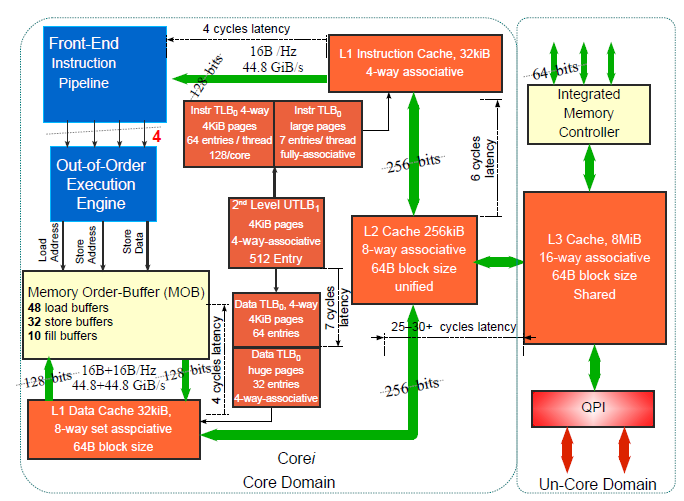
\includegraphics[width=0.80\linewidth]{fig/mem-nehalem-lat.png}

}

\end{frame}

\begin{frame}
\frametitle{Stránkování na 64-bitových architekturách}

Plná 64-bitová délka fyzické adresy nemá (zatím) použití.
Aní 64-bitová virtuální adresa. Úrovně zpomalují běh.
Nejvyšší bity se nahrazují znaménkvým rozšířením.
Horní oblast operační systém, spodní pro aplikace.
Další optimalizace volitelné velké stránky -- huge pages.

{
\centering

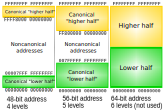
\includegraphics[width=0.6\linewidth]{paging-canonical-64-bit.pdf}

}
\end{frame}

\begin{frame}
\frametitle{Odkazy a literatura}

\begin{itemize}
\item Ulrich Drepper: \href{https://lwn.net/Articles/250967/}{What every programmer should know about memory}
\item Agner Fog: \href{https://www.agner.org/optimize/}{Software optimization resources. C++ and assembly}
\item \url{https://www.7-cpu.com/cpu/Haswell.html}
\item \url{https://www.7-cpu.com/cpu/Skylake.html}
\end{itemize}

\end{frame}

\begin{frame}
\frametitle{Prostor na poznámky}

\end{frame}

\end{document}

